\chapter{Implementierung}
\label{ch:implementierung}

% Neue Gliederung auf Grundlage des am 04.09.2026 gelesenen Quellcodes.
% Kapitel 2 erklärt die Verfahren, Kapitel 3 die Datengrundlage und Kapitel 4
% die Konzeption. Hier wird ausschließlich die konkrete Umsetzung beschrieben.
% Die Umsetzung der Validierung direkt bei der jeweiligen Komponente erklären,
% ohne einen eigenen Testabschnitt. Bereits in Kapitel 4 beschriebene Prüfziele,
% Testsignale und Vergleichsgrößen nur referenzieren. Hinzu kommen die konkrete
% Testumsetzung und ihre Grenzen. Ergebnisse und ihre Bewertung bleiben in 6.
% Die Erläuterungen unter den Überschriften sind Schreibhinweise, kein Fließtext.
% Falls Unterüberschriften nötig sind, unterhalb von \section ausschließlich
% unnummerierte \paragraphheading nutzen. Abschnitt 5.1 kommt ohne sie aus.
% Belege: konkrete Quellcodedateien und später vorhandene Anhangverweise;
% bei Fremdcode zusätzlich die ursprüngliche Quelle und die lokalen Änderungen.
% Keine Anhangnummern oder Quellcodeverweise erfinden.
% Der vorherige Kapiteltext ist außerhalb des Hauptdokuments gesichert unter
% tmp/ch5-vor-neugliederung-2026-09-04.tex.

%================================================================================================
%       5.1 Softwareumgebung
%================================================================================================
\section{Softwareumgebung}
\label{sec:softwareumgebung_impl}

% TABELLENVORSCHLAG: Python und die vier direkt verwendeten Bibliotheken
% mit Version und konkreter Aufgabe im Projekt kompakt gegenüberstellen.
% Grundlage: die unten bereits dokumentierten Softwarestände, Codefundstellen
% und offiziellen Dokumentationen. Bei der Überarbeitung Versionsangaben und
% wiederkehrende Aufgabenbeschreibungen in die Tabelle verlagern, nicht doppeln;
% Sprache und Bibliotheken weiterhin knapp in zusammenhängendem Text einordnen.
% Noch benötigt: Auswahl der knappen Zeileninhalte und Zuordnung ihrer Belege.

% Codebasis: cm_pipeline_validation/core/pipeline.py, run_pipeline;
% Rückverweis: Abschnitt~\ref{sec:verarbeitungspipeline_konzept}.
Der Prototyp setzt die konzipierte Verarbeitungspipeline in Python um.
% Quellenbasis: Python Software Foundation (2026), The Python Tutorial,
% Python 3.14.5 documentation, Einleitung, erste zwei Absätze nach dem
% Zielgruppenhinweis, unpaginiert: interpretierte Sprache, Standardbibliothek
% und zusätzlich verfügbare Module von Drittanbietern.
Python ist eine interpretierte Programmiersprache, für die neben der
Standardbibliothek zusätzliche Bibliotheken verfügbar sind
\cite{zotero-item-95}.

% Projektbasis: cm_pipeline_validation/README.md, Abschnitte "Dokumentierter
% Softwarestand" und "Installation und Einstieg"; .python-version;
% requirements.txt und requirements-lock.txt. Versionen am 04.09.2026 erneut
% mit .venv/bin/python und importlib.metadata.version geprüft.
Die am 4.~September~2026 erfasste Umgebung verwendet CPython~3.14.5
unter macOS~26.5.1 auf der Prozessorarchitektur arm64.
Die Python-Version ist in \path{.python-version} festgehalten. Die Datei
\path{requirements.txt} legt die nachfolgend genannten Versionen der vier
direkt verwendeten Bibliotheken fest. Ergänzend enthält
\path{requirements-lock.txt} den mit \texttt{pip freeze} erfassten
Paketbestand der lokalen virtuellen Umgebung einschließlich indirekter
Abhängigkeiten.

% Quellenbasis: NumPy Developers (o.J.), What is NumPy?, NumPy v2.4 Manual,
% erste zwei Absätze und "Why is NumPy fast?", unpaginiert: mehrdimensionale
% Arrays, elementweise Operationen, Fouriertransformationen und Statistik.
% Projektbasis der Version: requirements.txt, numpy==2.4.6.
Die numerische Grundlage bildet NumPy~2.4.6. Die Bibliothek stellt
mehrdimensionale Arrays bereit, also Datenfelder, deren Elemente einen
gemeinsamen Datentyp besitzen. Hinzu kommen mathematische Operationen auf
diesen Arrays sowie Funktionen für Fouriertransformationen und statistische
Berechnungen \cite{numpydevelopersWhatNumPy}.
% Codebasis: core/pipeline.py, PipelineResult und run_pipeline;
% core/drs.py, estimate_filter und apply_filter;
% core/fast_kurtogram.py, kurt und getFTSquaredEnvelope;
% core/envelope_analysis.py, compute_ses und _select_target_peak.
Im Prototyp liegen Zeitsignale, Frequenzachsen und Spektren als NumPy-Arrays
vor. Die Verarbeitung nutzt unter anderem elementweise Rechenoperationen,
die schnelle Fouriertransformation und die Bestimmung von Mittelwerten und
Medianen.

% Quellenbasis: The SciPy community (2026), SciPy documentation,
% SciPy v1.17.0 Manual, API reference: "Input and output (scipy.io)",
% Abschnitt "MATLAB files" (loadmat, whosmat), sowie "Signal processing
% (scipy.signal)", Abschnitte "Convolution" (oaconvolve), "Filtering"
% (lfilter), "Filter design" (firwin) und "Peak finding" (find_peaks),
% jeweils unpaginiert. Fundstellen: reference/io.html und reference/signal.html.
% Gegenprüfung mit den ausgelieferten Docstrings derselben Funktionen in
% SciPy 1.17.1 am 04.09.2026; keine Übernahme neuerer API-Eigenschaften.
% Projektbasis der Version: requirements.txt, scipy==1.17.1.
Für den Datenimport und weitere Signaloperationen kommt SciPy~1.17.1 hinzu.
Die Bibliothek bietet unter anderem Routinen zum Lesen von MATLAB-Dateien,
zur Faltung und digitalen Filterung sowie zur Suche nach Signalspitzen
\cite{thescipycommunitySciPyDocumentation2026}.
% Codebasis: utils/io.py, get_keys, load_signal_cwru und load_signal_paderborn;
% core/drs.py, apply_filter; core/fast_kurtogram.py, get_h_parameters,
% DBFB und TBFB; core/envelope_analysis.py, _find_spectrum_peaks.
Das Teilpaket \texttt{scipy.io} liest im Projekt die MAT-Dateien beider
Referenzdatensätze ein. Aus \texttt{scipy.signal} stammen die Faltung für die
DRS-Filterung, der Entwurf und die Anwendung der Filter des Fast Kurtograms
sowie die Bestimmung lokaler Maxima im \acrshort{SES}.

% Quellenbasis: The Matplotlib development team (o.J.), Quick start guide,
% Matplotlib 3.10.9 documentation, "A simple example", "Parts of a Figure",
% "Labelling plots" und "Color mapped data", unpaginiert: Diagramme,
% Achsen, Beschriftungen und farbcodierte Darstellung von Daten.
% Projektbasis der Version: requirements.txt, matplotlib==3.10.9.
Die grafische Darstellung übernimmt Matplotlib~3.10.9. Die Bibliothek bietet
Funktionen zum Erzeugen von Diagrammen mit beschrifteten Achsen sowie zur
farbcodierten Darstellung von Daten
\cite{thematplotlibdevelopmentteamQuickStartGuide}.
% Codebasis: utils/plot.py, drs_plot_time, drs_plot_spectra,
% plot_fast_kurtogram und plot_ses_with_faults; main.py und
% workflows/show_paderborn_example.py, jeweils main;
% core/pipeline.py, run_pipeline; core/fast_kurtogram.py, fast_kurtogram
% (Aufruf von Fast_Kurtogram mit verbose=False).
Im Projekt veranschaulicht sie die ursprünglichen und verarbeiteten
Zeitsignale, deren Spektren, das Kurtogramm und das \acrshort{SES} mit
eingezeichneten Lagerfrequenzen. Diese Grafiken dienen der Untersuchung
einzelner Messungen. Die automatisierten Verarbeitungsläufe erzeugen ihre
Ergebnisse ohne grafische Ausgabe.

% Quellenbasis: pandas (o.J.), 10 minutes to pandas, pandas 3.0.5 documentation,
% "Basic data structures in pandas", "Viewing data" (sort_values) und
% "Importing and exporting data -- CSV", unpaginiert: DataFrame als Tabelle,
% Sortierung sowie CSV-Ein-/Ausgabe. Gegenprüfung mit den ausgelieferten
% Docstrings von DataFrame, sort_values, read_csv und to_csv in pandas 3.0.3
% am 04.09.2026; die hier genannten Eigenschaften sind dort ebenfalls dokumentiert.
% Projektbasis der Version: requirements.txt, pandas==3.0.3.
Für die tabellarische Verarbeitung der Versuchsergebnisse wird
Pandas~3.0.3 verwendet. Mit dem \texttt{DataFrame} stellt die Bibliothek eine
zweidimensionale Datenstruktur mit Zeilen und Spalten bereit. Sie unterstützt
das Sortieren solcher Tabellen und den Datenaustausch über CSV-Dateien
\cite{pandas10MinutesPandas}.
% Codebasis: workflows/tune_paderborn.py, grid_search und main;
% workflows/evaluate_paderborn.py, load_trained_parameters, evaluate_files
% und main; workflows/evaluate_cwru.py, evaluate_files und main.
Die Parametersuche führt damit die geprüften Konfigurationen und ihre
Bewertungskennzahlen in einer Rangliste zusammen. Die Evaluationsskripte
lesen diese Liste wieder ein und übernehmen die an erster Stelle stehende
Konfiguration. Außerdem überführen sie die Resultate der einzelnen Messungen
und die zusammenfassenden Kennzahlen in Tabellen und speichern sie als
CSV-Dateien. Die Zuordnung dieser Aufgaben zu den konkreten Programmmodulen
beschreibt Abschnitt~\ref{sec:softwarestruktur}.

%================================================================================================
%       5.2 Programmaufbau
%================================================================================================
\section{Programmaufbau}
\label{sec:softwarestruktur}

% Rückverweis: Abschnitt~\ref{sec:verarbeitungspipeline_konzept}; der
% konzeptionelle Datenfluss wird vorausgesetzt, nicht erneut hergeleitet.
% Codebasis: cm_pipeline_validation/core/pipeline.py, run_pipeline;
% main.py, main; workflows/show_example.py, main;
% workflows/evaluate_paderborn.py und workflows/evaluate_cwru.py, evaluate_file.
Die in Abschnitt~\ref{sec:verarbeitungspipeline_konzept} entworfene Pipeline
ist in getrennten Python-Modulen umgesetzt. Dieselben Verarbeitungsfunktionen
werden für die grafische Untersuchung einzelner Messungen und für die
automatisierte Evaluation verwendet.

\paragraphheading{Module und Konfiguration}
\label{subsec:module_konfiguration_impl}

\begingroup
\setlength{\emergencystretch}{2em}

% Codebasis: cm_pipeline_validation/core/pipeline.py, run_pipeline;
% core/drs.py, run_drs; core/envelope_analysis.py, compute_ses und
% evaluate_spectrum; main.py, main; workflows/tune_paderborn.py, grid_search;
% workflows/evaluate_paderborn.py und workflows/evaluate_cwru.py, main.
Die Software ist überwiegend funktionsbasiert aufgebaut. Die
Verarbeitungskomponenten erhalten Signale und Parameter als Argumente und
geben ihre Ergebnisse an die aufrufende Funktion zurück.
\texttt{run\_pipeline} führt diese Komponenten für eine Messung zusammen;
die Auswahl mehrerer Dateien, die Auswertung der Versuche und die grafische
Darstellung liegen außerhalb dieser Funktion.
Abbildung~\ref{tab:modulorganisation_impl} zeigt die wesentlichen Module
und ihre Nutzungsabhängigkeiten.

% Codebasis der Abbildung: main.py, main und Importe;
% config/settings.py, Modulkonstanten; config/bearings.py,
% Geometrie-Dictionaries und get_paderborn_geometry;
% core/pipeline.py, run_pipeline und Importe; core/drs.py, run_drs;
% core/fast_kurtogram.py, fast_kurtogram und extract_band_envelope;
% core/envelope_analysis.py, compute_ses, compute_bearing_fault_frequencies
% und evaluate_spectrum; utils/io.py, load_signal_cwru,
% load_signal_paderborn und load_trained_parameters;
% utils/helper_functions.py, find_in_kwav; utils/plot.py, Grafikfunktionen;
% evaluation/paderborn_scope.py, collect_paderborn_files und expected_fault;
% evaluation/metrics.py, extract_detected_faults, diagnosis_metrics,
% detection_metrics; workflows/tune_paderborn.py, grid_search;
% workflows/evaluate_paderborn.py und workflows/evaluate_cwru.py,
% evaluate_files und Importe; workflows/show_example.py, main;
% workflows/run_complete_evaluation.py, STAGES und main.
\begin{figure}[htbp]
  \centering
  \input{pictures/module-components}
  \caption[Komponentendiagramm der Software]{Vereinfachtes
    Komponentendiagramm der Software. Die Pfeile zeigen
    ausgewählte Nutzungsabhängigkeiten und weisen auf die jeweils genutzte
    Komponente.}
  % Bestehendes Label der bisherigen Modulübersicht beibehalten.
  \label{tab:modulorganisation_impl}
\end{figure}

% Codebasis: tests/test_drs_synthetic_validation.py, DrsTest;
% tests/test_fast_kurtogram_reference.py, FastKurtogramReferenceTest;
% tests/test_ses.py, SquaredEnvelopeSpectrumTest;
% tests/test_peak_detection.py, PeakDetectionTest;
% tests/test_evaluation_scope.py, EvaluationScopeTest.
Ergänzend enthält \texttt{tests/} die automatisierten Prüfungen mit
\texttt{unittest}. Ihre konkrete Umsetzung wird bei den jeweiligen
Komponenten beschrieben.

% Codebasis: core/pipeline.py, run_pipeline, Z. 55--60 und 94--194;
% utils/io.py, load_signal_cwru und load_signal_paderborn: Rückgabe (signal, rpm).
Die zentrale Schnittstelle \texttt{run\_pipeline} in
\texttt{core/pipeline.py} erwartet den Pfad einer Messdatei, die Abtastrate,
ein Dictionary mit der Lagergeometrie sowie die DRS-Parameter und die
Zerlegungstiefe des Fast Kurtogram. Hinzu kommen benannte Argumente für
die Grenzen der Bandauswahl und die Konfiguration der Fehlerindikation.
Über \texttt{signal\_loader} lässt sich die Importfunktion übergeben; sie
liefert das Signal und die Drehzahl.
Der Schalter \texttt{use\_drs} bestimmt, ob die Signaltrennung verwendet
wird. Die Aufrufsignatur ist in
Listing~\ref{lst:pipeline-run-pipeline-schnittstelle} dokumentiert.

% Codebasis: core/pipeline.py, PipelineResult, Z. 20--52, und run_pipeline,
% Z. 180--194; core/fast_kurtogram.py, KurtogramResult und fast_kurtogram;
% utils/helper_functions.py, KurtogramBand und find_in_kwav.
Die Rückgabe ist in der mit \texttt{@dataclass} definierten Datenklasse
\texttt{PipelineResult} gebündelt.
Sie stellt die Drehzahl, das Eingangssignal und die Ergebnisse der
Signaltrennung bereit. Hinzu kommen das Kurtogramm mit seinen Achsen,
Mittenfrequenz und Bandbreite des ausgewählten Bandes, das SES mit
Frequenzachse sowie die berechneten Lagerfrequenzen und die Fehlerindikation.
Aufrufende Funktionen können diese Werte über benannte Felder wie
\texttt{result.ses} abrufen. Auch innerhalb der Verarbeitung bündeln
Datenklassen zusammengehörige Ausgaben: \texttt{KurtogramResult} enthält
das Kurtogramm und Angaben zu dessen globalem Optimum;
\texttt{KurtogramBand} beschreibt das unter den vorgegebenen Grenzen
ausgewählte Band. Diese Dataclasses dienen als Datencontainer für
zusammengehörige Ergebnisse, während die Berechnungen in Funktionen liegen.

% Codebasis: config/settings.py, DRS_PARAMS, NLEVEL, datensatzspezifische
% FS-/F_MIN-/F_MAX-Konstanten, MAX_BANDWIDTH und PADERBORN_* zur Datenauswahl;
% config/bearings.py, Geometrie-Dictionaries und get_paderborn_geometry;
% workflows/evaluate_paderborn.py, Importe und evaluate_file, Z. 80--98;
% core/pipeline.py, Importe und run_pipeline, Z. 124;
% core/envelope_analysis.py, compute_bearing_fault_frequencies.
Feste Einstellungen stehen in \texttt{config/settings.py}, Lagergeometrien
in \texttt{config/bearings.py}. Die Einstellungen umfassen unter anderem
Abtastraten, Grenzen der Bandauswahl, Vorgaben für DRS und Kurtogramm sowie
die Auswahl der Paderborner Messungen. Die Geometrieprofile bündeln
Wälzkörperzahl, Wälzkörper- und Teilkreisdurchmesser sowie Druckwinkel.
Für Paderborn ordnet \texttt{get\_paderborn\_geometry} der jeweiligen
Lagerkennung das hinterlegte Profil zu. \texttt{run\_pipeline} selbst
importiert diese Konfigurationsmodule nicht. Beispielsweise liest
\path{evaluate_paderborn.py} die Abtastrate und die Grenzen der Bandauswahl
aus \texttt{settings.py}, wählt das Geometrieprofil der Messung und
übergibt diese Werte an die Pipeline. Dort berechnet
\path{compute_bearing_fault_frequencies} aus der übergebenen Geometrie
und der eingelesenen Drehzahl die charakteristischen Lagerfrequenzen.

% Codebasis: workflows/show_example.py, DATA_PATH und main, Z. 29--89;
% utils/io.py, load_trained_parameters, Z. 93--155.
Für die manuelle Untersuchung einer einzelnen Messung dient
\texttt{workflows/show\_example.py}. Das Skript lädt die gespeicherten
Parameter der Parametersuche und verarbeitet die über den eingetragenen
Dateipfad ausgewählte Messung. Im aktuellen Stand ist dafür eine
CWRU-Messung mit Innenringschaden samt passender Abtastrate und
Lagergeometrie hinterlegt.
Anschließend übergibt das Skript die benötigten Ergebnisfelder an die
Grafikfunktionen für Zeitsignale, Spektren, Kurtogramm und SES.

% Codebasis: workflows/tune_paderborn.py, grid_search und main;
% utils/io.py, load_trained_parameters, Z. 93--155;
% core/drs.py, init_params, Z. 5--30;
% workflows/evaluate_paderborn.py und workflows/evaluate_cwru.py,
% evaluate_file und main; main.py, main.
Die Parameter für diese Einzeluntersuchung und die automatisierte Evaluation
werden aus derselben Ergebnisdatei geladen. \texttt{tune\_paderborn.py}
schreibt die Suchrangliste nach
\path{data/results/paderborn_param_search.csv}.
\path{load_trained_parameters} in \texttt{utils/io.py} übernimmt aus der
bestplatzierten Zeile die Zerlegungstiefe, die DRS-Parameter
sowie die Parameter der Fehlerindikation und ergänzt die weiteren festen
DRS-Vorgaben.
Listing~\ref{lst:evaluate-paderborn-load-trained-parameters-konfiguration}
zeigt die Zusammenstellung dieser Laufparameter.
Abtastrate, Lagergeometrie und Grenzen der Bandauswahl bestimmen die
Aufrufstellen weiterhin datensatzabhängig.

% Redaktionelle Zuordnung: Bedeutung und Auswahl der Parameter nach 4.4;
% Umrechnung in Blocklänge und Abstand nach 5.3, Detektorparameter nach 5.4.
% Der bereits in ch4.tex vorgemerkte Hinweis bleibt fachlich erforderlich:
% 3000 Hz ist laut Autor ein frei gewählter, nicht empirisch abgesicherter
% Schätzwert und keiner Literaturquelle entnommen. Die Korrelationsdauer
% wurde ebenfalls nicht aus den Messsignalen bestimmt. Grundlage:
% config/settings.py, DRS_PARAMS; workflows/tune_paderborn.py, grid_search;
% core/drs.py, init_params; Randall (2022), S. 277, Abschn. 7.3.2.
Die fachliche Bedeutung und Auswahl der Verarbeitungsparameter behandelt
Abschnitt~\ref{sec:parametrierungsstrategie}. Ihre Verwendung innerhalb
der Komponenten erläutern die Abschnitte~\ref{sec:signalverarbeitung_impl}
und~\ref{sec:signalbewertung_impl}.

% Codebasis: main.py, main, Z. 7--27;
% workflows/evaluate_paderborn.py, evaluate_file, Z. 86--100;
% workflows/evaluate_cwru.py, evaluate_file, Z. 155--169.
% Die methodische Begründung des Vergleichs steht in 4.5;
% die Umsetzung der Evaluationsläufe gehört nach 5.5.
Der Haupteinstiegspunkt \texttt{main.py} lädt die ausgewählte Konfiguration
und startet damit die Paderborn- und die CWRU-Evaluation, ohne die
Parametersuche erneut auszuführen. Für jeden Datensatz ruft er die
Evaluation mit \texttt{use\_drs=True} und \texttt{use\_drs=False} auf
(Listing~\ref{lst:main-main-einzelaufruf}) und speichert die Ergebnisse
in getrennten CSV-Dateien.
Die Evaluationsfunktionen übergeben die geladenen Parameter der
Fehlerindikation direkt an \texttt{run\_pipeline}.
Listing~\ref{lst:evaluate-paderborn-evaluate-file-parameteruebergabe} zeigt
diese Parameterübergabe über \texttt{**detection\_params} am
Paderborn-Aufruf.

% Codebasis: workflows/run_complete_evaluation.py, STAGES und main,
% Z. 9--24; workflows/evaluate_paderborn.py und workflows/evaluate_cwru.py,
% main und evaluate_files: use_drs=True als Vorgabe bei direktem Modulstart.
\path{workflows/run_complete_evaluation.py} bietet zusätzlich einen Ablauf
einschließlich neuer Parametersuche. Das Skript führt die Suche aus und
wertet anschließend die Paderborn- und CWRU-Messungen mit DRS aus.
\par\endgroup

\paragraphheading{Datenimport}
\label{sec:datenimport}

% Codebasis: utils/io.py, get_keys, load_signal_cwru und
% load_signal_paderborn; core/pipeline.py, run_pipeline, Importzweig und
% Rückgabeschnittstelle des Loaders.
Die beiden Importfunktionen in \texttt{utils/io.py} führen die
unterschiedlichen MAT-Strukturen auf dieselbe Schnittstelle zurück. Sie
liefern jeweils ein eindimensionales Schwingungssignal und einen einzelnen
Drehzahlwert. Tabelle~\ref{tab:datenimport_impl} bündelt die datensatzabhängige
Zuordnung dieser beiden Größen.

% Codebasis der Tabelle: utils/io.py, get_keys, load_signal_cwru und
% load_signal_paderborn.
\begin{table}[htbp]
  \centering
  \small
  \caption{Datensatzabhängige Zuordnung beim Datenimport}
  \label{tab:datenimport_impl}
  \begin{tabularx}{\textwidth}{|
      >{\raggedright\arraybackslash}p{2.0cm}|
      >{\raggedright\arraybackslash}X|
      >{\raggedright\arraybackslash}X|
      >{\raggedright\arraybackslash}p{3.0cm}|}
    \hline
    \textbf{Datensatz} & \textbf{Schwingungssignal} &
    \textbf{Drehzahl} & \textbf{Rückgabe} \\
    \hline
    CWRU & Variable mit der Endung \texttt{\_DE\_time}, zu einem
    eindimensionalen Array abgeflacht & Wert aus dem RPM-Feld; fehlt dieses,
    ein ausdrücklich übergebener Ersatzwert &
    Tupel \texttt{(signal, rpm)} aus Array und \texttt{float} \\
    \hline
    Paderborn & Nach Namen zugeordneter Kanal
    \texttt{vibration\_1}, zu einem eindimensionalen Array abgeflacht &
    Median des nach Namen zugeordneten Kanals \texttt{speed} &
    Tupel \texttt{(signal, rpm)} aus Array und \texttt{float} \\
    \hline
  \end{tabularx}
\end{table}

% Codebasis: core/pipeline.py, run_pipeline; config/settings.py,
% datensatzabhängige Abtastraten; config/bearings.py, Geometrieprofile;
% workflows/tune_paderborn.py, run_pipeline_file;
% workflows/evaluate_paderborn.py und workflows/evaluate_cwru.py,
% jeweils evaluate_file; evaluation/paderborn_scope.py, expected_fault;
% core/envelope_analysis.py, evaluate_spectrum.
Abtastrate und Lagergeometrie gehören nicht zur Rückgabe der Loader. Die
aufrufenden Workflows ergänzen beide Angaben beim Aufruf von
\texttt{run\_pipeline}. Die Workflows ermitteln die Referenzklasse außerhalb
des Imports; sie wird weder an die Importfunktion noch an die für die
Fehlerentscheidung zuständige Funktion \texttt{evaluate\_spectrum} übergeben.

% Quellenbasis: CWRU, o. J., Normal Baseline Data, Tabelle,
% Zeilen Normal_1/Normal_2, Spalte Approx. Motor Speed: 1772/1750 rpm.
% Codebasis: workflows/evaluate_cwru.py, NORMAL_RPM_IF_MISSING und
% evaluate_file; utils/io.py, load_signal_cwru. MAT-Header der vier
% lokalen Normaldateien geprüft: nur normal_1/2 ohne RPM-Feld.
Für \texttt{normal\_1.mat} und \texttt{normal\_2.mat} fehlen die RPM-Felder.
Der CWRU-Workflow übergibt deshalb die vom Datenanbieter angegebenen
ungefähren Drehzahlen von $1772$ beziehungsweise $1750\,\mathrm{min}^{-1}$
\cite{NormalBaselineData}. Diese Werte sind lokal hinterlegt; der Import
ruft die Website nicht ab. Ein vorhandenes RPM-Feld hat stets Vorrang.

% Codebasis: utils/io.py, load_signal_cwru und load_signal_paderborn;
% workflows/evaluate_paderborn.py, evaluate_file;
% tests/test_evaluation_scope.py,
% test_broken_paderborn_file_is_reported_instead_of_raising.
Fehlt bei CWRU das Drive-End-Signal oder sowohl das RPM-Feld als auch ein
Ersatzwert, bricht der Loader mit einem Fehler ab. Entsprechend führt ein
fehlender erforderlicher Paderborn-Kanal zu einem Importfehler. Der
Evaluationsworkflow fängt solche Fehler pro Datei ab und kennzeichnet den Lauf
als fehlerhaft. Der vorhandene Test mit einer beschädigten Paderborn-Datei
prüft ausschließlich diese Fehlerbehandlung des Workflows; er weist nicht die
fachliche Richtigkeit des Datenimports nach.

%================================================================================================
%       5.3 Signalverarbeitung
%================================================================================================
\section{Signalverarbeitung}
\label{sec:signalverarbeitung_impl}

% Dieser Abschnitt beschreibt, wie aus dem Messsignal das auszuwertende
% Spektrum entsteht. Keine erneute Herleitung der Methoden aus Kapitel 2.

% Rückverweis: Abschnitt~\ref{sec:verarbeitungspipeline_konzept};
% Codebasis: core/pipeline.py, run_pipeline, Z. 108--178.
Die Signalverarbeitung überführt die eingelesene Schwingungszeitreihe in
das \acrshort{SES} als Grundlage für die Fehlerindikation. Sie setzt damit den in
Abschnitt~\ref{sec:verarbeitungspipeline_konzept} beschriebenen Datenfluss
um. Im Mittelpunkt stehen hier die Verarbeitung der Signalarrays und die
Übergabe der Zwischenergebnisse zwischen den Komponenten.

\paragraphheading{DRS}
\label{subsec:drs_impl}

% Umsetzung in core/drs.py: Blocklänge und freier Abstand, Versatz N + delta,
% verzögerte Signalkopie, Hann-Fenster und Mittelung mehrerer Blockpaare.
% Schätzung des H1-Frequenzgangs, Filterung mit dessen Betrag mittels
% oaconvolve, zeitlich ausgerichteter Beschnitt und Bildung des Residuums.
% Die tatsächlichen Funktionsschritte erklären; Parameterwahl aus Kapitel 4
% nur referenzieren. Den Bypass use_drs=False in core/pipeline.py kurz nennen.
% Anschließend die Umsetzung der synthetischen Prüfung erläutern: Erzeugung
% und Mischung bekannter Signalanteile, Zuordnung der beschnittenen Ausgänge
% zu ihren Referenzen und automatisierte Prüfungen einschließlich reinem Rauschen.
% Testidee und Kennwertdefinitionen stehen bereits unter Komponentenvalidierung
% in Kapitel 4; hier auf die Testfunktionen und ihre konkreten Prüfgrenzen eingehen.
% Code: tests/test_drs_synthetic_validation.py. Ergebnisse nach Kapitel 6.

% Rückverweis: Abschnitt~\ref{sec:signalseparation}, DRS.
% Codebasis: core/drs.py, run_drs, Z. 129--164.
Die DRS zerlegt das Messsignal in einen geschätzten deterministischen
Anteil und ein Residuum (Abschnitt~\ref{sec:signalseparation}).
Die Funktion \texttt{run\_drs} in \texttt{core/drs.py} setzt dies in fünf
Schritten um: Bestimmung der DRS-Parameter, Erzeugung des verzögerten
Signals, Bestimmung des
$H_1$-Filters, Anwendung des Filters und Bildung des Residuums.
Sie erhält das Zeitsignal, die Abtastrate, die Drehzahl und die
DRS-Einstellungen aus der Laufkonfiguration.

% Rückverweis: Abschnitt~\ref{sec:parametrierungsstrategie}, Periodenbezug
% der Blocklänge und Abschätzung des freien Abstands.
% Codebasis: core/drs.py, init_params, Z. 25--30.
% resonance_freq ist ein vorgegebener Schätzwert, keine ermittelte Resonanz.
Zunächst berechnet \texttt{init\_params} die Blocklänge $N$ und
die freie Lücke $\Delta$ nach den Vorgaben aus
Abschnitt~\ref{sec:parametrierungsstrategie}. Als niedrigste
deterministische Frequenz wird die Wellenfrequenz angesetzt.
\texttt{n\_size} legt fest, wie viele Perioden dieser als niedrigste
deterministische Frequenz angesetzten Wellenfrequenz ein Analyseblock
umfasst. Die Lücke $\Delta$ wird anhand der angenommenen Resonanzfrequenz
\texttt{resonance\_freq} berechnet. Beide Zeitspannen werden mit der
Abtastrate in eine ganzzahlige Anzahl von Abtastwerten umgerechnet.

% Rückverweis: Gl.~\eqref{eq:drs_blocks}, freier Abstand und Blockversatz.
% Codebasis: core/drs.py, delay_signal, Z. 43--45; run_drs, Z. 149--160.
Anschließend erzeugt \texttt{delay\_signal} eine um $N+\Delta$ Abtastwerte
verzögerte Kopie. Dieser Versatz entspricht der Blockanordnung aus
Gleichung~\eqref{eq:drs_blocks}: Zwischen den beiden Blöcken der Länge $N$
bleibt die freie Lücke $\Delta$. Die am Anfang der Kopie eingefügten
Nullen werden bei der Filterbestimmung übersprungen.

% Rückverweis: Gl.~\eqref{eq:drs_h1_estimator}, H1-Schätzer und Mittelung;
% Abschnitt~\ref{par:spektraldarstellung_fensterung}, Fensterung.
% Codebasis: core/drs.py, estimate_filter, Z. 63--85; run_drs, Z. 154--160.
% Die Codevariablen A/B bezeichnen aktuellen/verzögerten Block.
% Es werden die Spektralprodukte und nicht blockweise berechnete H1-Filter gemittelt.
\texttt{estimate\_filter} setzt die Bestimmung des $H_1$-Filters aus
Gleichung~\eqref{eq:drs_h1_estimator} um. Dazu werden das ursprüngliche und
das verzögerte Signal in Blöcke der zuvor berechneten Länge $N$ aufgeteilt.
Da die FFT jeden endlichen Block als periodisch fortgesetzt behandelt,
können unterschiedliche Werte an seinen Rändern Sprünge und damit Leakage
im Frequenzbereich verursachen. Deshalb gewichtet die Funktion beide Blöcke
vor der FFT mit einem Hann-Fenster
(Abschnitt~\ref{par:spektraldarstellung_fensterung}). Anschließend mittelt
sie die für Zähler und Nenner von Gleichung~\eqref{eq:drs_h1_estimator}
benötigten Größen über alle Blockpaare und bildet daraus den Quotienten.

% Quellenbasis: Randall, Sawalhi und Coats (2011), S. 15, Abschn. 5:
% Verwendung der Amplitude des Frequenzgangs als Filtercharakteristik.
% Codebasis: core/drs.py, apply_filter, Z. 99--113;
% compute_residual, Z. 116--126; run_drs, Z. 162--164.
% Rückverweis: Abschnitt~\ref{sec:signalverarbeitung}, Absatz zur DFT:
% zyklische Anordnung der inversen DFT. Eigene Umsetzung mit fftshift und
% Beschnitt anhand des mittig angeordneten Nullzeitpunkts.
Für die Filteranwendung nutzt \texttt{apply\_filter} nur den Betrag
$\lvert H_1\rvert$. Damit wird die von Randall, Sawalhi und Coats
beschriebene amplitudenbasierte Variante umgesetzt
\cite[S.~15, Abschn.~5]{randallComparisonMethodsSeparation2011}.
Die inverse FFT des Betragsfilters liefert die Impulsantwort im Zeitbereich.
Da nur der Betrag des Filters verwendet wird, soll seine Impulsantwort
symmetrisch um den Zeitpunkt null liegen. Die inverse FFT ordnet die
zugehörigen Werte jedoch zyklisch an. \texttt{fftshift} verschiebt sie deshalb
vor der Faltung so, dass der Nullzeitpunkt in der Mitte liegt.
\texttt{oaconvolve} filtert das ursprüngliche Signal anschließend durch
lineare Faltung. Danach zieht \texttt{compute\_residual} den
geschätzten deterministischen Anteil vom Eingangssignal ab.
Zurückgegeben werden beide Signalanteile gleicher Länge sowie der
$H_1$-Frequenzgang und $N$.

% Bildgrundlage: vom Autor im aktuellen Auftrag bereitgestellte eigene
% Darstellung, unverändert übernommen aus
% codex-clipboard-2c631c1d-efb9-4253-bd70-152daf6a7f16.png.
% SHA-256: d009defd42af9b21c5ef6b25c05f8cb52a4d43e08aca91e099e706a980b6eb3c.
% Datenzuordnung laut Autor: PROJECT_ROOT / data/cwru/inner_race/IR007_2.mat.
Die Zuordnung von Eingangssignal, deterministischer Schätzung und
Residuum veranschaulicht Abbildung~\ref{fig:drs_signalanteile_impl}
an ihren Spektren.

\begin{figure}[htbp]
    \centering
    \includegraphics[width=\textwidth]{pictures/drs_signalanteile_autor.png}
    \caption{Spektren des Eingangssignals (oben), des geschätzten
    deterministischen Anteils (Mitte) und des Residuums (unten) für die
    CWRU-Messdatei \texttt{IR007\_2.mat}. Eigene Darstellung.}
    \label{fig:drs_signalanteile_impl}
\end{figure}

% Codebasis: core/pipeline.py, run_pipeline, Z. 55--60, 113--122, 135--153
% und 180--184; eingebundene Signatur in lst:pipeline-run-pipeline-schnittstelle.
In \texttt{run\_pipeline} wird das Residuum an Fast Kurtogram und
Hüllkurvenextraktion weitergegeben. Über \texttt{use\_drs=False}
lässt sich die standardmäßig aktive DRS abschalten
(Listing~\ref{lst:pipeline-run-pipeline-schnittstelle}).
Dann enthält \texttt{residual} eine Kopie des Rohsignals und
\texttt{filtered\_signal} nur Nullen; die nachfolgenden Schnittstellen
bleiben unverändert.

% Rückverweis: Abschnitt~\ref{sec:evaluationskonzept}, Komponentenvalidierung.
% Codebasis: tests/test_drs_synthetic_validation.py, create_deterministic_signal,
% Z. 26--39; create_random_components und create_random_signal, Z. 66--160;
% run_drs_case, Z. 218--260.
Die synthetische Prüfung aus Abschnitt~\ref{sec:evaluationskonzept}
ist in \path{tests/test_drs_synthetic_validation.py} umgesetzt.
\texttt{run\_drs\_case} mischt drei Sinusschwingungen mit einem zufälligen
Anteil aus Rauschen und einer Impulsfolge mit variierten Abständen und
Amplituden, die eine abklingende Resonanz anregt. Die vor der Mischung
gespeicherten Signalanteile dienen anschließend als Referenzen: Die
deterministische Schätzung wird
mit der Sinussumme verglichen, das Residuum mit dem gesamten zufälligen
Anteil einschließlich des Rauschens. Die Resonanzfrequenz wird bei
Signalerzeugung und DRS-Aufruf identisch vorgegeben.

% Codebasis: tests/test_drs_synthetic_validation.py, run_drs_case, Z. 254--297;
% DrsTest.test_drs_separates_known_signal_components, Z. 440--455.
% Rückverweis: Gl.~\eqref{eq:komponentenvalidierung_kennwerte}; keine neuen Definitionen.
\begingroup
\clubpenalty=10000
Für den Vergleich lässt der Test die Randbereiche am Anfang und Ende aus,
in denen die Faltung nicht vollständig durch Signaldaten gestützt ist.
Im verbleibenden Signalbereich vergleicht er den geschätzten
deterministischen Anteil und das Residuum mit ihren bekannten Referenzen.
Der Mischsignaltest fordert für beide Vergleiche Korrelationen größer als
$0{,}9$ und über das vollständige Signal einen Rekonstruktionsfehler kleiner
als $10^{-12}$. Zusätzlich werden der normierte \gls{RMSE} und das
Effektivwertverhältnis berechnet, jedoch ohne Bestehensgrenzen.
\par\endgroup

% Codebasis: tests/test_drs_synthetic_validation.py,
% DrsTest.test_white_noise_remains_in_residual, Z. 399--438.
Ein zweiter Test prüft bei ausschließlich weißem Rauschen, ob dieses
weitgehend im Residuum erhalten bleibt, und fordert dafür eine Korrelation
mit dem Eingangssignal größer als $0{,}98$. Zusätzlich vergleicht der Test
den über alle Frequenzstellen gemittelten Wert $\lvert H_1\rvert^2$ mit
$1/M$, wobei $M$ die Anzahl gemittelter Blockpaare bezeichnet; zugelassen ist
eine absolute Abweichung von $0{,}01$. Da die statistische Herleitung dieses
Referenzwerts für die aktuelle Blockbildung nicht dokumentiert ist, dient
diese Prüfung nicht als eigenständiger Nachweis der Trennqualität.
% Codebasis: tests/test_drs_synthetic_validation.py, run_drs_case, Z. 218--297,
% und DrsTest, Z. 399--455; core/drs.py, compute_residual, Z. 126.
% Aussagegrenzen des Referenzvergleichs, keine behaupteten Testergebnisse.
Die Prüfung erfasst damit ausgewählte synthetische Fälle, nicht die
ausgeschlossenen Signalränder oder die Folgen einer falsch angesetzten
Resonanzfrequenz. Der Rekonstruktionsfehler prüft lediglich, ob beide
zurückgegebenen Signalanteile zusammen wieder das Eingangssignal ergeben.
Da \texttt{compute\_residual} das Residuum als Differenz zwischen Eingang
und deterministischer Schätzung bildet, kann auch eine falsche Schätzung
diese Rekonstruktionsprüfung erfüllen. Die eigentliche Trennqualität
wird deshalb über den Vergleich mit den bekannten Referenzanteilen erfasst.
Ergebnisse und Bewertung folgen in Kapitel~\ref{ch:evaluation}.

\paragraphheading{Fast Kurtogram}
\label{subsec:fast_kurtogram_impl}

\begingroup
\setlength{\emergencystretch}{2em}

% Quellenbasis: T. Lecocq (Python-Übertragung 02/2012), Waveloc,
% PyProgs/kurtogram.py, Revision be1b744383d252b377b5311d09bad52d82df13c8,
% Fast_Kurtogram, Z. 163--265, sowie Filterbank- und Extraktionsfunktionen;
% LICENSE derselben Revision: CeCILL, Version 2.0, 2006.
% Originaldatei und Lizenz am 04.09.2026 direkt abgerufen und abgeglichen.
% Codebasis: core/fast_kurtogram.py, Herkunftskopf und markierter Kern,
% Z. 1--793; THIRD_PARTY_NOTICES.md, Abschnitt Waveloc / Python-Fast-Kurtogram.
% Rückverweis: Abschnitt~\ref{sec:bandauswahl}; keine erneute Theorie.
Die Implementierung in \path{core/fast_kurtogram.py} übernimmt die
Kurtogrammberechnung und die zugehörigen Filterbank- und
Extraktionsfunktionen aus dem GitHub-Repository Waveloc
\cite{lecocqFastKurtogram2012}. Die dortige Python-Fassung wurde von
T.~Lecocq auf Grundlage von J.~Antonis Algorithmus erstellt.
Die Waveloc-Anwendungsintegration wurde nicht übernommen. Der fremde Kern
und die eigenen Anpassungen sind im Modul gekennzeichnet; Herkunftshinweise
und CeCILL-Lizenz in Version~2.0 liegen dem Projekt bei.
% Literaturdaten am 04.09.2026 in Zotero ergänzt; den tatsächlich nach
% sources.bib exportierten Schlüssel lecocqFastKurtogram2012 verwendet.

% Codebasis: core/fast_kurtogram.py, get_h_parameters, Z. 63--73,
% raylinv, Z. 767--788; Abgleich mit den gleichnamigen Waveloc-Funktionen,
% Z. 58--66 und 809--829. Git-Nachweis der lokalen Anpassung:
% e71d2f60477b5fcc95fcc103d8a75edba8d21cd8, Autor levineckert, 03.09.2026.
% Codebasis: core/fast_kurtogram.py, _validate_fast_kurtogram_input,
% Z. 818--837; Waveloc, Fast_Kurtogram, Z. 210--226;
% matlab/Fast_Kurtogram.m, Z. 18--29.
% Codebasis der Schnittstellenzeile: core/fast_kurtogram.py,
% KurtogramResult, fast_kurtogram und extract_band_envelope, Z. 803--932.
Die wesentlichen eigenen Anpassungen fasst
Tabelle~\ref{tab:fast_kurtogram_anpassungen_impl} zusammen. Die rekursive
Filterbankzerlegung und die Kurtosisberechnung bleiben im übernommenen Kern.

\begin{table}[htbp]
  \centering
  \small
  \caption{Wesentliche eigene Anpassungen des Fast Kurtogram}
  \label{tab:fast_kurtogram_anpassungen_impl}
  \begin{tabularx}{\textwidth}{|
      >{\raggedright\arraybackslash}p{2.1cm}|
      >{\raggedright\arraybackslash}X|
      >{\raggedright\arraybackslash}X|}
    \hline
    \textbf{Bereich} & \textbf{Änderung} & \textbf{Zweck} \\
    \hline
    Kern & NumPy-Datentypfehler bei der Berechnung der Filterkoeffizienten
    behoben; in \texttt{raylinv} die Rückgabewerte für die Eingaben 0 und 1
    korrigiert. &
    Kompatibilität mit aktuellem NumPy herstellen und für diese Grenzwerte
    0 beziehungsweise unendlich zurückgeben. \\
    \hline
    Eingabe & Prüfung von Signal, Abtastrate und Zerlegungstiefe;
    Mittelwertentfernung vor der Filterbank. &
    Unzulässige Eingaben abweisen und die in Waveloc fehlende
    Zentrierung gemäß MATLAB-Routine ergänzen. \\
    \hline
    Schnittstelle & Strukturierte Ergebnisse und gezielte Bandextraktion
    mit Bandangaben in Hertz. &
    Kurtogramm und ausgewähltes Band für die Pipeline bereitstellen. \\
    \hline
  \end{tabularx}
\end{table}

% Codebasis: core/fast_kurtogram.py, KurtogramResult und fast_kurtogram,
% Z. 803--888; Fast_Kurtogram, Z. 163--289;
% core/pipeline.py, run_pipeline, Z. 113--145.
Für die Einbindung in die Pipeline wurde mit \texttt{fast\_kurtogram} ein
eigener Wrapper um die übernommene Waveloc-Funktion
\texttt{Fast\_Kurtogram} ergänzt. Er ruft den übernommenen Algorithmus ohne
grafische Ausgabe auf, prüft und zentriert das Eingangssignal und bündelt
Kurtogrammmatrix, Achsen und Bandangaben in einem strukturierten Ergebnis.
Die Pipeline übergibt dafür das Residuum beziehungsweise bei deaktivierter
DRS das Messsignal, die Abtastrate und die Zerlegungstiefe.

% Codebasis: core/pipeline.py, run_pipeline, Z. 124--145;
% core/envelope_analysis.py, DIAGNOSTIC_FAULT_TYPES, Z. 8;
% utils/helper_functions.py, find_in_kwav, Z. 71--164.
% Rückverweis: Absatz~\hyperref[par:auswahl_frequenzband]
% {Auswahl des Frequenzbandes} in Abschnitt~\ref{sec:methodenauswahl};
% dortige Auswahlbegründung und konkrete Parameter werden nicht wiederholt.
Das Ergebnis enthält außerdem Mittenfrequenz und Bandbreite des globalen
Maximums der Kurtogrammmatrix. In dieses Maximum gehen die
projektspezifischen Kriterien aus dem Absatz
\hyperref[par:auswahl_frequenzband]{Auswahl des Frequenzbandes} in
Abschnitt~\ref{sec:methodenauswahl} noch nicht ein. Deshalb durchsucht die
ergänzte Funktion \texttt{find\_in\_kwav} die berechnete Matrix und wählt das
stärkste Band, das alle vorgegebenen Bedingungen erfüllt. Für die
Mittenfrequenz gelten die Grenzen \texttt{f\_min} und \texttt{f\_max}; die
Bandbreite muss zwischen der berechneten Mindestbandbreite und
\texttt{max\_bandwidth} liegen
(Listing~\ref{lst:pipeline-run-pipeline-schnittstelle}). Die
Mindestbandbreite wird so festgelegt, dass das anschließende SES die BPFO-
und BPFI-Frequenzen einschließlich der mit \texttt{n\_harmonics}
berücksichtigten Harmonischen abdecken kann. Die ungefilterte Ebene null ist
ausgeschlossen, und die Bandränder müssen innerhalb des Nyquist-Intervalls
liegen. Erfüllt kein Band die Bedingungen, bricht die Auswahl ab.
% Detailnachweis im vorgesehenen Auswahl-Listing: nextafter setzt die
% Mindestbandbreite auf die nächstgrößere Gleitkommazahl; die Auswahlhilfe
% berücksichtigt replizierte Matrixspalten, endliche Kurtosiswerte und eine
% numerische Randtoleranz. Diese Routinedetails werden hier nicht ausgeführt.

% Eigene Darstellung auf Grundlage des aktuellen Pipelineaufrufs:
% workflows/show_example.py, DATA_PATH und main, Z. 32--75;
% utils/plot.py, plot_fast_kurtogram, Z. 8--75.
% Abgebildetes Ergebnis: data/results/cwru_paderborn_params_results.csv,
% Zeile IR014_3.mat: fc = 4500 Hz, bw = 1000 Hz.
Abbildung~\ref{fig:fast_kurtogram_ir014_3} veranschaulicht die
Kurtogrammmatrix und die anschließende Bandauswahl am Beispiel der
CWRU-Messdatei \texttt{IR014\_3.mat}. Die horizontale Achse zeigt die
Frequenz in Hertz, die vertikale Achse die Zerlegungsstufen. Mit steigender
Zerlegungsstufe werden schmalere Frequenzbänder untersucht; die Farbe gibt
den Wert der spektralen Kurtosis an. Die grauen gepunkteten Linien markieren
den zulässigen Frequenzbereich von 500 bis 5000\,Hz. Die weiße gestrichelte
Linie kennzeichnet die gewählte Mittenfrequenz von 4500\,Hz, der weiße
Rahmen das ausgewählte Band von 4000 bis 5000\,Hz.

\begin{figure}[htbp]
  \centering
  \includegraphics[width=\textwidth]{fast_kurtogram_ir014_3_autor.png}
  \caption[Fast Kurtogram der Messdatei IR014\_3.mat]{Fast Kurtogram mit
    Bandauswahl für \texttt{IR014\_3.mat}. Eigene Darstellung.}
  \label{fig:fast_kurtogram_ir014_3}
\end{figure}

% Codebasis: core/fast_kurtogram.py, extract_band_envelope, Z. 891--932,
% Find_wav_kurt, Z. 594--619, K_wpQ_filt und K_wpQ_filt_local;
% core/pipeline.py, run_pipeline, Z. 146--178 und 188--189;
% core/envelope_analysis.py, compute_ses, Signatur und Z. 36--41.
Der übernommene Waveloc-Aufruf berechnet die komplexe Hüllkurve zunächst nur
für das globale Maximum. Da \texttt{find\_in\_kwav} ein anderes Band wählen
kann, wurde \texttt{extract\_band\_\allowbreak envelope} ergänzt. Die Funktion enthält
keinen neu entwickelten Filteralgorithmus, sondern ruft für das ausgewählte
Band die übernommene Funktion \texttt{Find\_wav\_kurt} auf. Die Pipeline
prüft, ob deren Bandangaben der zuvor ausgewählten Kurtogrammzelle
entsprechen. Anschließend übergibt sie die komplexe Hüllkurve zusammen mit
der Bandbreite an \texttt{compute\_ses}. Mittenfrequenz und Bandbreite des
ausgewählten Bandes bleiben im Pipelineergebnis gespeichert.
% Details der Schnittstelle: Die Extraktion entfernt ebenso wie die
% Kurtogrammberechnung den Mittelwert des Eingangssignals. center_frequency
% wird für die vorhandene Funktion Find_wav_kurt durch fs geteilt; dies
% ist eine Umrechnung zwischen Schnittstellen, kein neuer Filterschritt.
% run_pipeline prüft Mittenfrequenz und Bandbreite mit np.isclose und
% bricht bei unpassenden Bandangaben ab. detect_faults=False überspringt
% nur die anschließende Fehlerentscheidung; Extraktion und SES bleiben aktiv.

% Quellenbasis: J. Antoni (2015), Fast Kurtogram, MATLAB Central File
% Exchange 48912, Version 1.0.0.0, Rubriken Overview und Version History;
% Originalarchiv Version 1, Fast_Kurtogram.m, Dateikopf (Revision 12/2014),
% numerischer Hauptteil und Unterfunktionen. Am 04.09.2026 direkt gelesen
% und mit der lokalen Datei verglichen; license.txt stimmt byteweise mit
% LICENSES/Antoni-Fast-Kurtogram.txt überein (Copyrightjahr dort: 2014).
% Codebasis: matlab/Fast_Kurtogram.m, Fast_Kurtogram, Z. 1 und 44--56;
% lokaler Git-Nachweis: 4406f7553c80fe26e32f979b29c8f97bd341883a.
% Rückverweis: Abschnitt~\ref{sec:evaluationskonzept}, Komponentenvalidierung.
% Codebasis der Prüfgrößen: tests/test_fast_kurtogram_reference.py,
% test_python_matches_matlab_reference, Z. 65--96. Die Einordnung der
% Rundungsunterschiede wird aus sec:evaluationskonzept aufgegriffen.
Zur Überprüfung der Python-Fassung werden ihre Ergebnisse für ausgewählte
Paderborner Messungen mit Antonis ursprünglicher MATLAB-Implementierung
\cite{antoniFastKurtogram2015} verglichen. Geprüft werden alle Werte der
Kurtogrammmatrix sowie Mittenfrequenz und Bandbreite des globalen Maximums.
Die Werte müssen innerhalb der in Abschnitt~\ref{sec:evaluationskonzept}
festgelegten Toleranzen übereinstimmen, die kleine numerische Abweichungen
etwa durch Rundungen zulassen.

% Codebasis: matlab/Fast_Kurtogram.m, Fast_Kurtogram, Z. 1 und 44--56;
% Originalabgleich und Lizenznachweis siehe Quellenkommentar oben.
Für den automatisierten Vergleich wurde die MATLAB-Funktion so ergänzt,
dass sie diese Ergebnisse direkt zurückgibt, ohne Abbildungen zu öffnen
oder Benutzereingaben anzufordern. Die numerischen Filterbank-Unterfunktionen
blieben unverändert. Die zugehörige BSD-Lizenz mit zwei Bedingungen liegt
dem Projekt bei.
% Literaturdaten am 04.09.2026 in Zotero ergänzt; den tatsächlich nach
% sources.bib exportierten Schlüssel antoniFastKurtogram2015 verwendet.
% Codebasis: tests/create_fast_kurtogram_reference.m, Skript, Z. 5--100;
% config/settings.py, PADERBORN_EVALUATION_BEARINGS,
% PADERBORN_OPERATING_CONDITIONS und PADERBORN_RECORDING_NUMBERS;
% tests/test_fast_kurtogram_reference.py, selected_measurements,
% load_matlab_references und FastKurtogramReferenceTest, Z. 26--96;
% utils/io.py, load_signal_paderborn, Z. 81--90.
Das Skript \path{tests/create_fast_kurtogram_reference.m} berechnet die
MATLAB-Ergebnisse und speichert für jede Messung die Kurtogrammmatrix und
die Bandangaben zusammen mit ihrem Dateinamen in einer MAT-Datei. Der
Python-Test verwendet diesen Namen, um das MATLAB-Ergebnis genau derjenigen
Messdatei zuzuordnen, aus der es berechnet wurde. Vor dem Zahlenvergleich
prüft er außerdem, ob Referenzdatei und Konfiguration dieselbe Messauswahl,
Abtastrate und Zerlegungstiefe angeben.

% Codebasis: tests/test_fast_kurtogram_reference.py,
% FastKurtogramReferenceTest.test_python_matches_matlab_reference, Z. 65--96;
% tests/create_fast_kurtogram_reference.m, Z. 71--89;
% core/fast_kurtogram.py, _validate_fast_kurtogram_input und fast_kurtogram;
% matlab/Fast_Kurtogram.m, Z. 29--41.
% Rückverweis: Abschnitt~\ref{sec:evaluationskonzept}, Prüfgrößen und Toleranzen.
Beide Implementierungen verarbeiten den vollständigen Kanal
\texttt{vibration\_1} ohne DRS, mit Mittelwertentfernung vor der Filterbank
und übereinstimmenden Filtervorgaben. Python übernimmt Abtastrate und
Zerlegungstiefe aus der Referenzdatei.
% Testdetails für das vorgesehene Listing: assert_allclose prüft Matrix,
% Mittenfrequenz und Bandbreite; Zuordnung als subTest pro Datei;
% keine gesonderte Duplikatprüfung beim Aufbau des Referenz-Dictionarys;
% equal_nan=True akzeptiert übereinstimmende NaN-Positionen, ohne separate
% Endlichkeitsprüfung. Daraus wird keine allgemeine Korrektheit abgeleitet.

% Codebasis: tests/test_fast_kurtogram_reference.py, skipUnless,
% test_reference_contains_exactly_the_selected_measurements und
% test_python_matches_matlab_reference; MATLAB-Skript, Z. 59--61 und 77--79;
% matlab/Fast_Kurtogram.m, Z. 53--55: keine Hüllkurvenreferenz bei diesem Aufruf.
Fehlt die Referenzdatei, wird die Testklasse übersprungen; fehlende
Einzelreferenzen oder Messdateien lassen die Prüfung fehlschlagen.
Der Vergleich bezieht für diese Messungen den übernommenen Kurtogrammkern
und die im Wrapper ergänzte Mittelwertentfernung ein. Er prüft weder die
eingeschränkte Bandauswahl noch die Hüllkurvenwerte, das SES oder die gesamte
Pipeline.
% Ergebnisse und Bewertung bleiben Kapitel~\ref{ch:evaluation} vorbehalten.
\par\endgroup

\paragraphheading{SES}
\label{subsec:ses_impl}
% Keine Leerzeile vor dem Einstieg: Überschrift und Text zusammenhalten.
\begin{samepage}
% Den Übergang von der komplexen Hüllkurve zum Betragsspektrum beschreiben;
% Routinedetails der übernommenen Waveloc-Berechnung im Haupttext nicht
% einzeln ausführen. Die eigene Frequenzachse verständlich abgrenzen.
% Die Definition aus Kapitel 2 nicht wiederholen. Die spätere Umrechnung in
% Dezibel und die Peakbewertung gehören in Abschnitt 5.4.
% Code: core/fast_kurtogram.py (getFTSquaredEnvelope),
% core/envelope_analysis.py (compute_ses). Auch die übernommene SES-Routine
% ist als Fremdcode kenntlich zu machen.
% Validierung direkt anschließen: künstliche komplexe Hüllkurve mit bekannter
% Modulation; prüfen, ob das stärkste Maximum oberhalb von 0 Hz bei der
% vorgegebenen Frequenz liegt. Dieser Test prüft nicht die vollständige Bandauswahl.
% Code: tests/test_ses.py. Testergebnis nach Kapitel 6.
%
% Rückverweis: Abschnitt~\ref{sec:huellkurvenanalyse}, insbesondere
% Gl.~\eqref{eq:squared_envelope} und \eqref{eq:squared_envelope_spectrum};
% die dortige Definition wird vorausgesetzt, nicht erneut hergeleitet.
% Codebasis: core/pipeline.py, run_pipeline, Z. 162--165 und 180--194;
% core/envelope_analysis.py, compute_ses, Z. 11--44.
% Routineprüfung für den Codeanhang: bandwidth <= 0 führt vor der
% Berechnung zu einem ValueError (compute_ses, Z. 32--33).
Nachdem das Fast Kurtogram die komplexe Hüllkurve des ausgewählten Bandes
bereitgestellt hat, berechnet die Funktion \texttt{compute\_ses} daraus das
in Abschnitt~\ref{sec:huellkurvenanalyse} eingeführte \acrshort{SES}. Die
Pipeline übergibt zusätzlich die Bandbreite des ausgewählten Bandes und
erhält ein Betragsspektrum mit zugehöriger Frequenzachse zurück.
\par\end{samepage}

% Quellenbasis: T. Lecocq (Python-Übertragung 02/2012), Waveloc,
% PyProgs/kurtogram.py, Revision be1b744383d252b377b5311d09bad52d82df13c8,
% getFTSquaredEnvelope, Z. 615--629; Autorenhinweise in Fast_Kurtogram,
% Z. 173--174; LICENSE derselben Revision, Schlusszeile: CeCILL 2.0 (2006).
% Originalfundstellen am 04.09.2026 über GitHub direkt geprüft.
% Codebasis: core/fast_kurtogram.py, getFTSquaredEnvelope, Z. 622--636:
% Funktionskörper mit der Originalfundstelle textuell abgeglichen;
% core/envelope_analysis.py, compute_ses, Z. 32--44;
% THIRD_PARTY_NOTICES.md, Abschnitt Waveloc / Python-Fast-Kurtogram.
% Rückverweis zur bereits offengelegten Herkunft und Lizenz:
% subsec:fast_kurtogram_impl; dessen Waveloc-Quellenfußnote gilt auch hier.
Für die Spektralberechnung ruft \texttt{compute\_ses} die Waveloc-Routine
\texttt{getFTSquaredEnvelope} auf. Sie wurde unverändert aus T.~Lecocqs
Python-Übertragung des Algorithmus von J.~Antoni übernommen. Die Routine
bildet das Betragsquadrat der komplexen Hüllkurve und bestimmt daraus mit
einer Fourier-Transformation das Spektrum.
Ihre Herkunft und die CeCILL-Lizenz in Version~2.0 sind im Absatz
\hyperref[subsec:fast_kurtogram_impl]{Fast Kurtogram} ausgewiesen.

% Codebasis: core/fast_kurtogram.py, getFTSquaredEnvelope, Z. 632--636,
% sowie nextpow2, Z. 32--45. Rückverweis zu FFT und Fensterung:
% Abschnitt~\ref{sec:signalverarbeitung}; keine neue Wirkungsbehauptung.
% Funktionsdetails für den Codeanhang: np.hanning erzeugt das Fenster;
% nextpow2 bestimmt die FFT-Länge.
Die aus Waveloc übernommene Routine liefert die Beträge des vollständigen
FFT-Arrays, jedoch keine Frequenzachse in Hertz. Die eigene Funktion
\texttt{compute\_ses} ergänzt deshalb die für die Pipeline benötigte
Frequenzzuordnung. Dazu setzt sie die effektive Abtastrate der Hüllkurve auf
das Doppelte der übergebenen Bandbreite und berechnet daraus die
Frequenzbins.

% Codebasis: core/envelope_analysis.py, compute_ses, Z. 35--44;
% core/fast_kurtogram.py, getFTSquaredEnvelope, Z. 632--636.
% Abgleich der Abtastrate mit dem ausgeführten Filterbankpfad:
% DBFB, Z. 512--520; TBFB, Z. 545--558; Find_wav_kurt, Z. 594--610;
% K_wpQ_filt und K_wpQ_filt_local, Z. 686--753;
% extract_band_envelope, Z. 915--932; core/pipeline.py, run_pipeline,
% Z. 154--165 und 180--194 (Ergebnisfelder).
% Rasterbezug: Gl.~\eqref{eq:dft_frequency_grid}; hier bezogen auf die
% tatsächlich verwendete FFT-Länge einschließlich etwaiger Nullauffüllung.
% Funktionsdetails für den Codeanhang: np.fft.rfftfreq erzeugt die Achse;
% Auswahl der ersten nfft // 2 + 1 Spektralwerte. PipelineResult speichert
% die Rückgabe in freq_ses und ses.
Die Rückgabe enthält nur den bei 0~Hz beginnenden Teil des Spektrums bis zur
Bandbreite des ausgewählten Bandes. Dies ist mit dem einseitigen Spektrum
gemeint; die zweite Hälfte des vollständigen FFT-Arrays wird nicht
weitergegeben.

% Rückverweis: Abschnitt~\ref{sec:evaluationskonzept}, Komponentenvalidierung:
% getrennte Prüfung der Softwarekomponenten; dort steht bislang kein
% konkreter SES-Prüffall. Die folgenden Angaben stammen aus dem Testcode.
% Codebasis: tests/test_ses.py, SquaredEnvelopeSpectrumTest,
% test_known_modulation_appears_at_the_expected_frequency, Z. 13--33.
% Technische Prüfdetails für den Codeanhang: frequency > 0 maskiert den
% Gleichanteil; np.argmax wählt den größten Wert, assertEqual prüft die
% exakte Gleichheit von Peak- und Modulationsfrequenz.
Die getrennte Komponentenprüfung aus
Abschnitt~\ref{sec:evaluationskonzept} wird für das SES durch einen
synthetischen Test in \path{tests/test_ses.py} umgesetzt. Er erzeugt 1024
Werte bei einer Hüllkurvenabtastrate von 1024~Hz und bildet damit genau eine
Sekunde ab. Da die verwendete FFT ebenfalls 1024 Punkte umfasst, liegen die
Frequenzbins im Abstand von 1~Hz. Als bekanntes Ziel wird eine
quadrierte Hüllkurve mit einer Kosinusmodulation bei 64~Hz vorgegeben. Vor
dem Aufruf von \texttt{compute\_ses} zieht der Test daraus elementweise die
Quadratwurzel, weil die übernommene Routine den Betrag der komplexen
Hüllkurve intern wieder quadriert. Dadurch liegt vor der
Fourier-Transformation erneut genau die vorgegebene Modulation vor. Der
Test prüft anschließend, ob der stärkste Spektralwert oberhalb von 0~Hz
exakt dem Frequenzbin bei 64~Hz zugeordnet wird.

% Codebasis der Prüfgrenzen: tests/test_ses.py, einziger Prüffall,
% Z. 13--33, insbesondere Erzeugung in Z. 15--22 und Assertion in Z. 33.
% Keine Ergebnisaussage: beschrieben werden ausschließlich Prüfkriterium
% und nicht geprüfte Eigenschaften; Testergebnisse gehören in Kapitel 6.
% Weitere Grenzen dieses einzelnen Prüffalls: Nur 64 Hz auf dem FFT-Raster,
% ausschließlich reelle Werte trotz komplexen Datentyps und eine Länge,
% die bereits eine Zweierpotenz ist. Andere Frequenzen, Eingaben mit
% Imaginäranteil und das Auffüllen mit Nullen werden nicht geprüft.
Damit prüft der Test, ob die SES-Implementierung eine gezielt erzeugte,
ideal auf dem Frequenzraster liegende Modulation an der vorgegebenen Stelle
wiederfindet. Er vergleicht weder das vollständige Spektrum noch dessen
absolute Werte mit einer Referenz. Auch die Bandauswahl und die Gewinnung
der komplexen Hüllkurve sind nicht abgedeckt, da der Test unmittelbar an
der Schnittstelle von \texttt{compute\_ses} ansetzt.

% Bildgrundlage: vom Autor im aktuellen Auftrag bereitgestellte eigene
% Darstellung, unverändert übernommen aus
% codex-clipboard-32d33912-a729-4fed-82bb-563ae6b02284.png.
% SHA-256: b11f9acd03bd5e0e7737facec6a46ec3856845870e462f940831f8ea4d3580d7.
% Datenzuordnung und Darstellungslogik im aktuellen Projektarbeitsstand:
% workflows/show_example.py, PADERBORN_EXAMPLE und main, Z. 38--45 sowie
% 140--149; utils/plot.py, plot_ses_with_faults, Z. 213--260.
% Die Abbildung dient der Veranschaulichung der Ausgabe, nicht als Ergebnis-
% oder Gütenachweis.
\begin{figure}[H]
  \noindent Ein Beispiel für das von der Pipeline zurückgegebene SES mit
  eingezeichneten charakteristischen Lagerfrequenzen ist in
  Abbildung~\ref{fig:ses_n15_m07_f10_ka04_20} dargestellt. Die blaue Kurve
  zeigt das SES; die gestrichelten Linien markieren die Sollfrequenzen für
  BPFO und BPFI sowie deren im Plot berücksichtigte ganzzahlige Vielfache.
  \par\medskip
  \centering
  \includegraphics[width=\textwidth]{pictures/ses_n15_m07_f10_ka04_20_autor.png}
  \caption[SES der Messdatei N15\_M07\_F10\_KA04\_20.mat]{SES der
    Paderborner Messdatei
    \path{N15_M07_F10_KA04_20.mat} für eine Mittenfrequenz
    von 10\,000~Hz und eine Bandbreite von 1\,333~Hz mit eingezeichneten
    BPFO- und BPFI-Sollfrequenzen. Eigene Darstellung.}
  \label{fig:ses_n15_m07_f10_ka04_20}
\end{figure}

%================================================================================================
%       5.4 Signalbewertung
%================================================================================================
\section{Signalbewertung}
\label{sec:signalbewertung_impl}

% Rückverweis: Abschnitt~\ref{sec:verarbeitungspipeline_konzept} und Absatz
% \hyperref[par:fehlerindikation_pipeline]{Fehlerindikation}; keine neue
% externe Aussage. Codebasis: core/pipeline.py, run_pipeline, Z. 108--178.
Die Signalbewertung verbindet das zuvor berechnete \acrshort{SES} mit der
Drehzahl und der Lagergeometrie. Sie berechnet daraus zunächst die
Sollfrequenzen und wendet anschließend die in Absatz
\hyperref[par:fehlerindikation_pipeline]{Fehlerindikation} festgelegte Regel
auf das Spektrum an. So entsteht die Fehlerindikation für eine einzelne
Messung.

\paragraphheading{Lagerfrequenzen}
\label{subsec:lagerfrequenzen_impl}

% Datengrundlage: technische Begleitunterlagen der Datensätze; für CWRU
% Bearing Information des Bearing Data Center, für Paderborn die lokalen
% Lagerdatenblätter, unter anderem KA04.pdf und KA05.pdf.
% Interne Primärgrundlage: cm_pipeline_validation, core/pipeline.py,
% run_pipeline, Z. 108--124; config/bearings.py, Geometrieprofile und
% get_paderborn_geometry, Z. 4--69; workflows/evaluate_cwru.py, evaluate_file,
% Z. 153--169; workflows/evaluate_paderborn.py, evaluate_file, Z. 80--98.
\texttt{run\_pipeline} übernimmt die vom Signalimport gelieferte Drehzahl und
ein von der Aufrufstelle gewähltes Geometrie-Dictionary. Dieses enthält die
Wälzkörperzahl, den Wälzkörper- und Teilkreisdurchmesser sowie den
Druckwinkel. Die im Code hinterlegten Geometrieprofile basieren auf den
technischen Begleitunterlagen der jeweiligen Datensätze. Die CWRU-Aufrufe
verwenden das hinterlegte Geometrieprofil des Lagertyps~6205. Bei den
Paderborner Messungen liest die Aufrufstelle die Lagerkennung aus dem
Verzeichnispfad; \texttt{get\_paderborn\_geometry} ordnet ihr eines der
hinterlegten Geometrieprofile des Lagertyps~6203 zu.

% Rückverweis: Absatz
% \hyperref[par:charakteristische_lagerschadensfrequenzen]
% {Charakteristische Lagerschadensfrequenzen}; Formeln, Größen und fachliche
% Zuordnung sind dort bereits eingeführt und werden hier nicht wiederholt.
% Interne Primärgrundlage: cm_pipeline_validation,
% core/envelope_analysis.py, compute_bearing_fault_frequencies, Z. 47--69,
% DIAGNOSTIC_FAULT_TYPES, Z. 8, und evaluate_spectrum, Z. 174--228;
% core/pipeline.py, run_pipeline, Z. 124--129 und 167--178.
Die Funktion \texttt{compute\_bearing\_fault\_frequencies} wandelt die
Drehzahl in Umdrehungen pro Minute in die Wellenrotationsfrequenz in Hertz um
und setzt mit den Geometrieparametern die im Absatz
\hyperref[par:charakteristische_lagerschadensfrequenzen]
{Charakteristische Lagerschadensfrequenzen} eingeführten Beziehungen
programmatisch um. Ihr Rückgabewert enthält BPFO, BPFI, BSF und FTF. Die
anschließende Fehlerentscheidung verwendet im aktuellen Code dagegen nur BPFO
und BPFI.

% Rückverweis: Abschnitt~\ref{sec:evaluationskonzept}, Komponentenvalidierung.
% Interne Primärgrundlage: cm_pipeline_validation,
% tests/test_peak_detection.py,
% test_fault_frequencies_match_independent_reference_values, Z. 130--149.
% Die Vergleichswerte wurden mit den in Kapitel 2 eingeführten Beziehungen für
% dieselben Eingaben berechnet und auf zwei Nachkommastellen gerundet.
Der automatisierte Test in \path{tests/test_peak_detection.py} setzt diese
Prüfung mit zwei Fällen um: Er übergibt für CWRU eine Drehzahl von
1797~U/min und das 6205-Profil, für Paderborn 1500~U/min und das hinterlegte
MTK-/IBU-6203-Profil. Für den Test wurden die BPFO- und BPFI-Vergleichswerte
mit den in Kapitel~2 eingeführten Beziehungen für die jeweiligen Drehzahlen und
Geometrieprofile berechnet und auf zwei Nachkommastellen gerundet. Da der Test
die beiden Geometrie-Dictionaries direkt auswählt, prüft er weder BSF und FTF
noch die vollständige Zuordnung der Geometrieprofile zu den Paderborner
Lagerkennungen.

\paragraphheading{Peak-Erkennung}
\label{subsec:peaks_impl}

% Rückverweis: Absatz
% \hyperref[par:fehlerindikation_pipeline]{Fehlerindikation}; die methodische
% Begründung der lokalen Peakprüfung ist dort bereits enthalten.
% Interne Primärgrundlage: cm_pipeline_validation,
% core/envelope_analysis.py, _find_spectrum_peaks, Z. 72--77,
% _select_target_peak, Z. 80--127, detect_local_peak, Z. 130--171, sowie
% evaluate_spectrum, Z. 223--244.
Die Peak-Erkennung prüft, ob das \acrshort{SES} in der Umgebung einer
berechneten Sollfrequenz ein lokales Maximum enthält, das sich ausreichend vom
lokalen Hintergrund abhebt. Die Implementierung teilt diesen Lösungsweg auf
zwei Hilfsfunktionen auf: \texttt{\_find\_spectrum\_peaks} bereitet das
Spektrum einmalig auf und bestimmt sämtliche lokalen Maxima.
\texttt{\_select\_target\_peak} wählt daraus für eine Sollfrequenz einen
Kandidaten aus und bewertet ihn. \texttt{detect\_local\_peak} verbindet beide
Schritte für einen einzelnen Aufruf. Bei der Auswertung mehrerer
Sollfrequenzen verwendet \texttt{evaluate\_spectrum} die einmal ermittelten
Maxima erneut. Abbildung~\ref{fig:peakpruefung_ablauf} zeigt den Ablauf von der
Eingabe des \acrshort{SES} bis zum Gültigkeitsstatus des Peaks.

% Eigene Darstellung auf Grundlage der internen Primärgrundlage
% cm_pipeline_validation, core/envelope_analysis.py,
% _find_spectrum_peaks, Z. 72--77, und _select_target_peak, Z. 80--127.
\begin{figure}[htbp]
  \centering
  \resizebox{\textwidth}{!}{%
    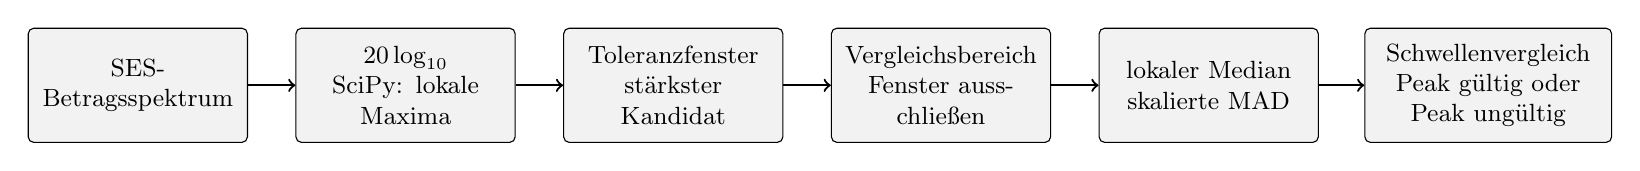
\begin{tikzpicture}[
        block/.style={
          draw,
          rounded corners=2pt,
          fill=black!5,
          align=center,
          minimum height=1.45cm,
          text width=2.55cm,
          font=\small
        }
      ]
      \node[block] (ses) at (0,0) {SES-\\Betragsspektrum};
      \node[block] (maxima) at (3.4,0)
        {$20\log_{10}$\\SciPy: lokale Maxima};
      \node[block] (candidate) at (6.8,0)
        {Toleranzfenster\\stärkster Kandidat};
      \node[block] (surrounding) at (10.2,0)
        {Vergleichsbereich\\Fenster ausschließen};
      \node[block] (mad) at (13.6,0)
        {lokaler Median\\skalierte MAD};
      \node[block, text width=2.9cm] (result) at (17.15,0)
        {Schwellenvergleich\\Peak gültig oder\\Peak ungültig};

      \draw[->, line width=0.8pt] (ses.east) -- (maxima.west);
      \draw[->, line width=0.8pt] (maxima.east) -- (candidate.west);
      \draw[->, line width=0.8pt] (candidate.east) -- (surrounding.west);
      \draw[->, line width=0.8pt] (surrounding.east) -- (mad.west);
      \draw[->, line width=0.8pt] (mad.east) -- (result.west);
    \end{tikzpicture}%
  }
  \caption{Ablauf der implementierten Einzelpeakprüfung}
  \label{fig:peakpruefung_ablauf}
  \caption*{\footnotesize Quelle: eigene Darstellung.}
\end{figure}

% Interne Primärgrundlage: cm_pipeline_validation,
% core/envelope_analysis.py, _find_spectrum_peaks, Z. 72--77, sowie
% evaluate_spectrum, Z. 223--244.
Die Hilfsfunktion \texttt{\_find\_spectrum\_peaks} bereitet das Spektrum vor.
Zunächst wandelt sie dessen Werte mit $20\log_{10}$ in Dezibel
um. Für zwei positive Amplituden $A_1$ und $A_2$ erscheint ihr Verhältnis
dadurch als Differenz
$20\log_{10}(A_1/A_2)$. Die Bewertung berücksichtigt damit relative
Unterschiede zum lokalen Hintergrund statt nur den absoluten numerischen
Abstand auf der linearen Skala. Vor dem Logarithmieren ersetzt die Funktion
Nullwerte durch eine kleine positive Gleitkommazahl, um den Wert $-\infty$ zu
vermeiden. Anschließend nutzt sie die Funktion \texttt{find\_peaks} aus dem
SciPy-Modul \texttt{scipy.signal}, um sämtliche lokalen Maxima des
umgerechneten Spektrums zu bestimmen. Die zurückgegebenen Indizes werden für
die Prüfung der Sollfrequenzen weiterverwendet, aber nicht gespeichert.

% Rückverweis: Absatz
% \hyperref[par:fehlerindikation_pipeline]{Fehlerindikation}; dort sind die
% schlupfbedingte Frequenzabweichung, das relative Toleranzfenster, der lokale
% Vergleich sowie die Skalierung der MAD mit 1,4826 bereits erklärt und belegt.
% Interne Primärgrundlage: cm_pipeline_validation,
% core/envelope_analysis.py, _select_target_peak, Z. 80--127.
Für jede Sollfrequenz bildet \texttt{\_select\_target\_peak} zunächst das
relative Toleranzfenster. Wie im Absatz
\hyperref[par:fehlerindikation_pipeline]{Fehlerindikation} erläutert, lässt
dieses Fenster Abweichungen zwischen berechneter und tatsächlicher
Lagerfrequenz zu, die unter anderem durch Schlupf entstehen können. Unter den
lokalen Maxima im Fenster wählt die Funktion den Kandidaten mit dem größten
linearen SES-Wert. Um ihn mit seiner Umgebung zu vergleichen, betrachtet sie
den durch \texttt{freq\_search\_area} festgelegten Bereich beiderseits der
Sollfrequenz und schließt das Toleranzfenster daraus aus. Reicht dieser Bereich
unter 0~Hz, beginnt er bei 0~Hz, da das einseitige \acrshort{SES} keine
negativen Frequenzen enthält.

Aus allen verbleibenden Dezibelwerten berechnet die Funktion den lokalen
Median und die skalierte MAD. Der dafür verwendete Faktor $1{,}4826$ ist
bereits im Absatz
\hyperref[par:fehlerindikation_pipeline]{Fehlerindikation} eingeführt und
belegt. Die Differenz zwischen dem Kandidaten und dem lokalen Median wird durch
die skalierte MAD geteilt. Der entstehende MAD-Score gibt damit an, um wie
viele skalierte MAD der Kandidat über dem lokalen Median liegt. Erreicht der
Score mindestens den Wert des Parameters $k$, gilt der Peak als gültig.

% Interne Primärgrundlage: cm_pipeline_validation,
% core/envelope_analysis.py, _select_target_peak, Z. 94--126.
Die Implementierung behandelt drei Sonderfälle. Enthält das Toleranzfenster
kein lokales Maximum, liegt kein Peakkandidat vor und die Prüfung ist negativ.
Bleiben nach dem Ausschluss des Toleranzfensters weniger als drei
Vergleichswerte übrig, verwirft die Funktion den Kandidaten, statt aus dieser
kleinen Menge eine lokale Schwelle zu bestimmen. Beträgt die MAD null, etwa bei
einem vollständig konstanten Vergleichsbereich, ist die Division zur Bildung
des Scores nicht möglich. Die Funktion akzeptiert den Kandidaten dann nur,
wenn er strikt über dem lokalen Median liegt.

% Interne Primärgrundlage: cm_pipeline_validation,
% tests/test_peak_detection.py, PeakDetectionTest, Z. 18--99, insbesondere
% detected_faults und Fälle mit gesetzten Peaks, Z. 25--67,
% test_no_fault_is_detected, Z. 45--48,
% test_spectral_slope_is_not_a_peak, Z. 69--82, und
% test_isolated_peak_is_valid_when_local_mad_is_zero, Z. 84--99.
% Keine Ergebnisaussage: Hier werden nur Aufbau und Aussagegrenzen der
% technischen Prüfungen beschrieben; die Resultate gehören in Kapitel 6.
Zur technischen Validierung der Funktionsweise erzeugt die Testklasse mehrere
künstliche Spektren auf einem Frequenzraster von 0 bis 250~Hz in Schritten von
1~Hz. Für den Grundfall klarer Peaks innerhalb der Zielfenster hebt eine
Hilfsfunktion auf einem konstanten Hintergrund einzelne Frequenzpositionen auf
den Wert 10 an. Je nach Testfall liegen diese Maxima bei 50 und 100~Hz, bei 70
und 140~Hz oder in beiden Gruppen. Da diese Fälle
\texttt{evaluate\_spectrum} aufrufen, prüfen sie zugleich die anschließende
Fehlerentscheidung; für die Peak-Erkennung decken sie die Auswahl klar
isolierter Kandidaten innerhalb der Fenster ab.

Weitere Tests behandeln die Randfälle der Kandidatensuche. Peaks bei 52 und
104~Hz liegen außerhalb der eng um 50 und 100~Hz gesetzten Zielfenster und
prüfen deren Ausschluss. Ein monoton von 1 auf 2 ansteigendes Spektrum besitzt
kein lokales Maximum und prüft, ob ein steigender Verlauf allein als Peak
zurückgewiesen wird. Für den Fall einer MAD von null setzt ein Test bei 50~Hz
einen einzelnen Wert von 2 auf einen sonst konstanten Hintergrund von 1. Die
Prüfungen beschränken sich damit auf exakt im 1-Hz-Raster platzierte und stark
vereinfachte Verläufe. Sie bilden weder realistische Rausch- und
Seitenbandstrukturen noch mehrere nahe beieinanderliegende Kandidaten oder
Peaks zwischen den Frequenzstellen ab. Für den Sonderfall mit weniger als drei
Vergleichswerten enthält die Testdatei keinen eigenen Test. Die Ergebnisse
werden in Kapitel~\ref{ch:evaluation} berichtet.

\paragraphheading{Fehlerentscheidung}
\label{subsec:fehlerentscheidung_impl}

% Interne Primärgrundlage: cm_pipeline_validation,
% core/envelope_analysis.py, DIAGNOSTIC_FAULT_TYPES, Z. 8, und
% evaluate_spectrum, Z. 174--270, insbesondere Schleife über Fehlerarten und
% Frequenzordnungen Z. 223--256 sowie Entscheidungsverknüpfung Z. 258--269.
% Rückverweis: Absatz
% \hyperref[par:fehlerindikation_pipeline]{Fehlerindikation}; dort ist die
% gemeinsame Einordnung der getrennten BPFO-/BPFI-Ergebnisse bereits
% beschrieben. Keine neue externe Aussage.
% Implementierungsabweichung: run_pipeline, Z. 101--106, und evaluate_spectrum,
% Z. 216--220, erzwingen derzeit n_harmonics >= 2 und
% 2 <= required_harmonics <= n_harmonics. Die Prüfung dieser festen
% Eingabeschranken ist in der BA-To-do-Datei vorgemerkt und wird hier nicht als
% methodische Festlegung dargestellt.
Die Peak-Erkennung liefert für jede untersuchte Frequenz die Information, ob
dort ein gültiger Peak vorliegt. Aus diesen Ergebnissen leitet die
Fehlerentscheidung getrennt für BPFO und BPFI ab, ob ein Schaden angezeigt
wird. Die Implementierung erreicht dies in drei Schritten:
Sie legt die zu prüfenden Frequenzen fest, verknüpft die gültigen Peaks zu je
einem Ergebnis für BPFO und BPFI und speichert diese Ergebnisse zusammen mit
den Einzelbefunden. Diese Aufgaben übernimmt die Funktion
\texttt{evaluate\_spectrum}.

Im ersten Schritt prüft die Funktion für BPFO und BPFI jeweils die
Grundfrequenz $f$ und ihre ganzzahligen Vielfachen. Wie viele Frequenzen sie
insgesamt untersucht, legt \texttt{n\_harmonics} fest; die Grundfrequenz zählt
dabei bereits mit. Bei \texttt{n\_harmonics}$=5$ werden somit $f$, $2f$, $3f$,
$4f$ und $5f$ geprüft.

Im zweiten Schritt zählt die Funktion die gültigen Peaks. Der Parameter
\texttt{required\_\allowbreak harmonics} gibt an, wie viele der untersuchten Frequenzen
einschließlich der Grundfrequenz gültig sein müssen. Für eine Indikation müssen
zwei Bedingungen erfüllt sein: Die Grundfrequenz muss einen gültigen Peak
aufweisen und die Gesamtzahl gültiger Peaks muss mindestens
\texttt{required\_\allowbreak harmonics} entsprechen. Die Entscheidung erfolgt für BPFO
und BPFI getrennt. Welche Fehlerindikation sich aus diesen beiden Prüfungen
ergibt, erläutert der
\hyperref[par:fehlerindikation_pipeline]{Absatz \emph{Fehlerindikation}}.

% Interne Primärgrundlage: cm_pipeline_validation,
% core/envelope_analysis.py, _select_target_peak, Z. 90--127, und
% evaluate_spectrum, Z. 230--270, insbesondere Berechnung von error_pct,
% Detail-Dictionary und Ergebnis-Dictionary, Z. 246--269.
% Begriffsabgrenzung: Die relative Frequenzabweichung dokumentiert die im Code
% gespeicherte Differenz von Ziel- und Kandidatenfrequenz relativ zur
% Zielfrequenz. Sie dient zusammen mit dem Toleranzfenster zur Berücksichtigung
% möglicher Verschiebungen, isoliert deren Ursache jedoch nicht. Rückverweise:
% \hyperref[par:fehlerindikation_pipeline]{Fehlerindikation} zum Schlupf,
% Gl.~\eqref{eq:dft_frequency_grid} zum diskreten Frequenzraster sowie
% Absatz~\ref{subsec:peaks_impl} zur Auswahl des Peakkandidaten.
Im dritten Schritt erstellt die Funktion die Rückgabe. Für BPFO und BPFI hält
sie fest, ob ein Schaden angezeigt wird und wie viele der untersuchten
Frequenzen einen gültigen Peak besitzen. Hinzu kommt eine Liste der
Einzelprüfungen. Jeder Eintrag enthält die berechnete Zielfrequenz, die Frequenz
des ausgewählten Peakkandidaten, dessen Spektralwert und MAD-Score, die relative
Frequenzabweichung und die Angabe, ob der Peak gültig ist. Die Funktion prüft
und dokumentiert alle mit \texttt{n\_harmonics} festgelegten Frequenzen, auch
wenn sie dort keinen gültigen Peak findet. Liegt im Zielfenster kein lokales
Maximum, trägt sie für Kandidatenfrequenz, Spektralwert, MAD-Score und relative
Frequenzabweichung jeweils null ein und kennzeichnet den Eintrag als ungültig.

Für einen ausgewählten Kandidaten zeigt die relative Frequenzabweichung in
Prozent, wie weit seine Frequenz von der Zielfrequenz entfernt liegt. Sie dient
damit auch dazu, Frequenzverschiebungen durch Schlupf zu berücksichtigen. Der
Wert kann jedoch nicht allein dem Schlupf zugerechnet werden, da auch die
Frequenzauflösung des Spektrums und die Auswahl des Peakkandidaten die
Abweichung beeinflussen.

% Interne Primärgrundlage: cm_pipeline_validation,
% tests/test_peak_detection.py, PeakDetectionTest, Entscheidungsfälle
% Z. 45--67 und Variation von required_harmonics Z. 101--128;
% tests/test_evaluation_scope.py,
% test_only_inner_and_outer_race_faults_are_evaluated, Z. 29--44.
% Beschrieben werden Zusammenhang, Testumfang und Prüfziel, keine
% Testergebnisse.
Die Entscheidung hängt nicht von einem einzelnen Peak ab, sondern von der
Kombination der Grundfrequenz mit weiteren Vielfachen. Die Tests prüfen daher,
ob die Funktion verschiedene Kombinationen gültiger Peaks wie vorgesehen
auswertet. Die Testklasse in
\path{tests/test_peak_detection.py} erzeugt dazu künstliche Spektren für die
Fälle ohne Indikation, nur mit BPFO, nur mit BPFI und mit beiden Schadensarten.
Ein weiterer Test variiert \texttt{required\_\allowbreak harmonics} und prüft damit, ob die
festgelegte Mindestzahl gültiger Peaks die Entscheidung steuert. Ein separater
Test in \path{tests/test_evaluation_scope.py} übergibt neben BPFO und BPFI auch
BSF und FTF als Sollfrequenzen. Damit wird geprüft, dass die Funktion trotzdem
nur BPFO und BPFI auswertet. Diese Fälle prüfen die Umsetzung der
Entscheidungsregel. Ihre Anwendung auf die Messdaten und die daraus folgende
Bewertung werden in Kapitel~\ref{ch:evaluation} behandelt.

%================================================================================================
%       5.5 Versuchsautomatisierung
%================================================================================================
\section{Versuchsautomatisierung}
\label{sec:versuchsautomatisierung}

% Umsetzung der Versuchsskripte einschließlich zugehöriger Prüfungen,
% nicht die Ergebnisdarstellung oder deren Bewertung.
% Kennzahlen zuerst erklären, weil die Parametersuche sie zur Rangbildung nutzt.

% Eigene Implementierungsübersicht: cm_pipeline_validation,
% evaluation/metrics.py, diagnosis_metrics und detection_metrics;
% workflows/tune_paderborn.py, grid_search und main;
% utils/io.py, load_trained_parameters;
% workflows/evaluate_paderborn.py und workflows/evaluate_cwru.py, jeweils
% evaluate_files und main; workflows/run_complete_evaluation.py, main.
Die Versuchsumgebung übernimmt drei aufeinander aufbauende Aufgaben. Zunächst
werden Referenzklassen und Fehlerindikationen in einheitliche Kennzahlen
überführt. Diese Kennzahlen dienen anschließend dazu, die
Parameterkonfigurationen anhand der Paderborner Trainingsdaten zu ordnen. Die
bestplatzierte Konfiguration wird danach für die getrennten Evaluationsläufe
mit den Paderborner Evaluationsdaten und dem CWRU-Datensatz geladen.

\paragraphheading{Kennzahlen}
\label{subsec:kennzahlen_impl}

% evaluation/metrics.py: extract_detected_faults bildet Klassenmengen und
% ordnet eine leere Erkennung normal zu. diagnosis_metrics und
% detection_metrics vergleichen die Ausgaben mit den bekannten Referenzklassen.
% Bildung und Aggregation der Zählwerte, exakte Übereinstimmung und Behandlung
% leerer Nenner mit safe_divide erklären. Definitionen aus Kapitel 4 nur
% referenzieren. metrics.py führt keine Peak-Erkennung durch.
% Die nicht verwendete Hilfsfunktion score_faults nicht als Bestandteil der
% aktuellen Parametersuche darstellen.
% Keine eigenständige Validierung der Kennzahlen behaupten, solange dafür
% keine konkrete Prüfung vorliegt; Tests der Fehlerentscheidung ersetzen sie nicht.

% Rückverweis: Absatz \enquote{Bewertungskennzahlen} in
% Abschnitt~\ref{sec:evaluationskonzept}; keine erneute Definition oder
% Begründung der Kennzahlen.
% Interne Primärgrundlage: cm_pipeline_validation,
% core/envelope_analysis.py, DIAGNOSTIC_FAULT_TYPES und evaluate_spectrum,
% Z. 8 und 174--270; evaluation/metrics.py, extract_detected_faults, Z. 26--43.
Die Kennzahlenberechnung hat das Ziel, die Referenzklasse jeder einbezogenen
Messung und die von der Pipeline erkannten Fehlerklassen in einheitliche
Kennzahlen zu überführen. Die Auswahl, fachliche Bedeutung und mathematische
Definition dieser Kennzahlen
sind bereits im Absatz
\hyperref[sec:evaluationskonzept]{\enquote{Bewertungskennzahlen}} in
Abschnitt~\ref{sec:evaluationskonzept} festgelegt. Für jede Messung liest
\texttt{extract\_\allowbreak detected\_\allowbreak faults} die Ergebnisse der
Fehlerentscheidung für BPFO und BPFI aus. Ist BPFO als erkannt markiert, nimmt
die Funktion die Klasse \texttt{BPFO} in die Ergebnismenge auf; für BPFI
verfährt sie ebenso. Liegt keine der beiden Fehlerindikationen vor, enthält die
Ergebnismenge stattdessen ausschließlich die Klasse \texttt{normal}. Damit
steht für jede Messung eine Menge erkannter Klassen bereit, die sowohl für die
binäre Schadenserkennung als auch für die Klassenzuordnung verwendet wird.

% Interne Primärgrundlage: cm_pipeline_validation, evaluation/metrics.py,
% diagnosis_metrics und safe_divide, Z. 46--96.
Für die Klassenzuordnung vergleicht \texttt{diagnosis\_metrics} bei jeder
Messung die erkannten Klassen mit der zugehörigen Referenzklasse. Enthält das
Ergebnis die Referenzklasse, erhöht die Funktion \gls{TP}; fehlt sie, erhöht
die Funktion \gls{FN}. Jede weitere erkannte Klasse erhöht \gls{FP}. Die
Funktion summiert diese drei Zählwerte über alle Messungen. Zusätzlich erfasst
sie eine exakte Übereinstimmung, wenn das Ergebnis ausschließlich die
Referenzklasse enthält. Aus den summierten Werten berechnet sie die dort
festgelegten Kennzahlen der Klassenzuordnung sowie den Anteil der exakten
Übereinstimmungen.

% Interne Primärgrundlage: cm_pipeline_validation, evaluation/metrics.py,
% detection_metrics, Z. 99--149, und safe_divide, Z. 46--56.
Für die binäre Schadenserkennung betrachtet \texttt{detection\_metrics} nicht
die konkrete Fehlerklasse, sondern nur, ob Referenz und Ergebnis einen Schaden
anzeigen. Eine Referenzklasse ungleich \texttt{normal} gilt als Schaden. Eine
Ergebnismenge mit BPFO, BPFI oder beiden Klassen gilt ebenfalls als Schaden;
\texttt{normal} steht für keinen erkannten Schaden. Die Funktion ordnet jede
Messung anhand dieses Vergleichs \gls{TP}, \gls{TN}, \gls{FP} oder \gls{FN}
zu und summiert die vier Zählwerte. Daraus berechnet sie die Kennzahlen der
binären Schadenserkennung. Die von beiden Berechnungsfunktionen verwendete
Hilfsfunktion \texttt{safe\_divide} gibt bei einem Nenner von null den Wert
\texttt{0.0} zurück.

% Interne Primärgrundlage: cm_pipeline_validation,
% workflows/tune_paderborn.py, evaluate_detection, Z. 132--188;
% workflows/evaluate_paderborn.py, evaluate_file und evaluate_files,
% Z. 58--112 und 128--198; workflows/evaluate_cwru.py, evaluate_file und
% evaluate_files, Z. 122--182 und 199--276.
Die Parametersuche berechnet beide Kennzahlengruppen für jede Konfiguration
mit \texttt{diagnosis\_\allowbreak metrics} und
\texttt{detection\_\allowbreak metrics}. Nach demselben Ablauf berechnen die
Evaluationsskripte die Kennzahlen für die Paderborner und die CWRU-Messungen.
Somit verwenden Parametersuche und Evaluation dieselben Berechnungsregeln.

\paragraphheading{Parametersuche}
\label{subsec:parametersuche_impl}

% Rückverweis: Abschnitt~\ref{sec:parametrierungsstrategie}; Auswahl und
% fachliche Bedeutung der Parameter, Datentrennung und Suchraum werden nicht
% erneut begründet. Interne Primärgrundlage: cm_pipeline_validation,
% workflows/tune_paderborn.py, grid_search und main, Z. 191--285.
Ziel der Parametersuche ist es, alle vorgesehenen Konfigurationen anhand der
Paderborner Trainingsdaten zu bewerten, ohne die rechenintensive
Signalverarbeitung für jede reine Detektorkombination zu wiederholen.
Dazu bildet das Suchskript die Parameterkombinationen und berechnet zunächst
die gemeinsam nutzbaren Spektren. Diese werden zwischengespeichert und mit
den zugehörigen Detektoreinstellungen erneut bewertet. Aus den Kennzahlen
aller Kombinationen entsteht anschließend eine Rangliste, die als CSV-Datei
gespeichert wird. Abbildung~\ref{fig:parametersuche_ablauf} zeigt die Trennung
der beiden Verarbeitungsschritte.

% Eigene Darstellung auf Grundlage der internen Primärgrundlage
% cm_pipeline_validation, workflows/tune_paderborn.py, run_pipeline_cache,
% evaluate_detection, grid_search und main, Z. 96--188 und 191--284.
\begin{figure}[htbp]
  \centering
  \resizebox{\textwidth}{!}{%
    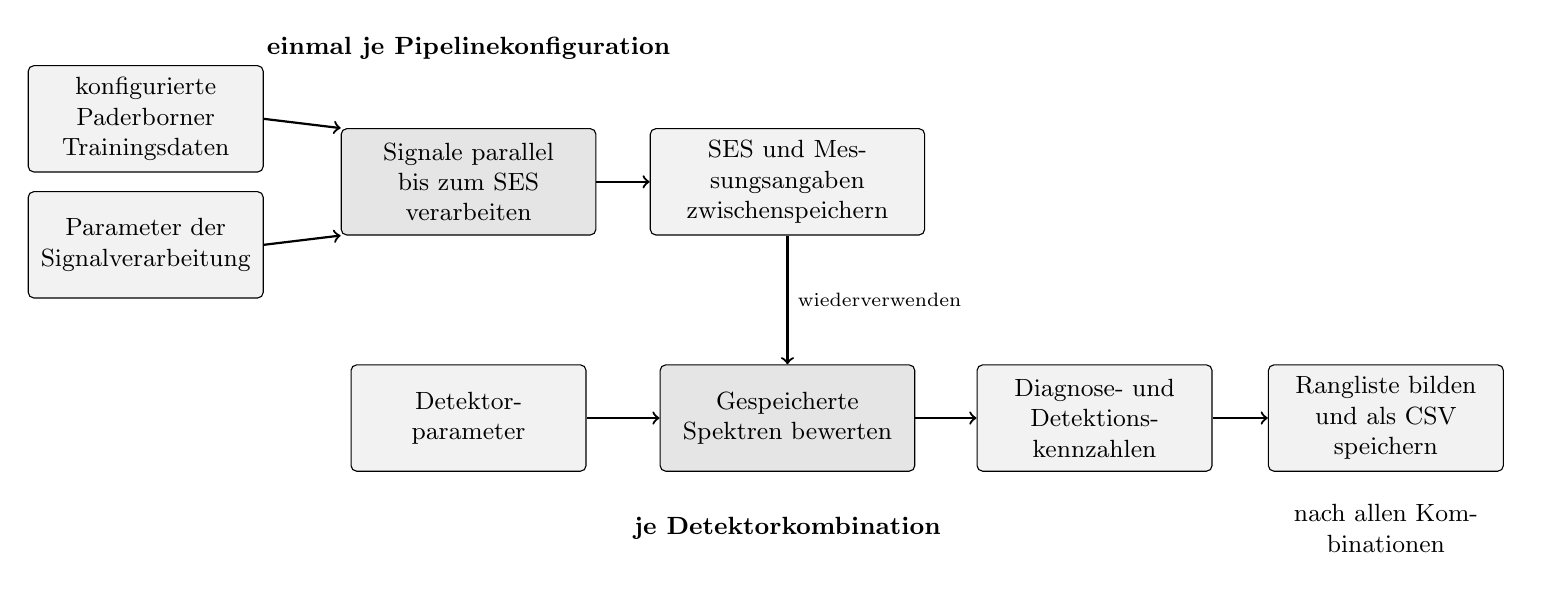
\begin{tikzpicture}[
        block/.style={
          draw,
          rounded corners=2pt,
          fill=black!5,
          align=center,
          minimum height=1.35cm,
          text width=2.75cm,
          font=\small
        },
        phase/.style={block, fill=black!10, text width=3.0cm}
      ]
      \node[font=\small\bfseries] at (4.1,3.05)
        {einmal je Pipelinekonfiguration};
      \node[block] (files) at (0,2.15)
        {konfigurierte Paderborner\\Trainingsdaten};
      \node[block] (pipelineparams) at (0,0.55)
        {Parameter der\\Signalverarbeitung};
      \node[phase] (pipeline) at (4.1,1.35)
        {Signale parallel\\bis zum SES\\verarbeiten};
      \node[block, text width=3.25cm] (cache) at (8.15,1.35)
        {SES und Messungsangaben\\zwischenspeichern};

      \node[font=\small\bfseries] at (8.15,-3.05)
        {je Detektorkombination};
      \node[block] (detectorparams) at (4.1,-1.65)
        {Detektor-\\parameter};
      \node[phase] (evaluation) at (8.15,-1.65)
        {Gespeicherte\\Spektren bewerten};
      \node[block] (metrics) at (12.05,-1.65)
        {Diagnose- und\\Detektions-\\kennzahlen};
      \node[block] (ranking) at (15.75,-1.65)
        {Rangliste bilden\\und als CSV speichern};
      \node[font=\small, text width=3.2cm, align=center] at (15.75,-3.05)
        {nach allen Kombinationen};

      \draw[->, line width=0.8pt] (files.east) -- (pipeline.north west);
      \draw[->, line width=0.8pt] (pipelineparams.east) -- (pipeline.south west);
      \draw[->, line width=0.8pt] (pipeline.east) -- (cache.west);
      \draw[->, line width=0.8pt] (detectorparams.east) -- (evaluation.west);
      \draw[->, line width=0.8pt] (cache.south) -- node[right, font=\scriptsize]
        {wiederverwenden} (evaluation.north);
      \draw[->, line width=0.8pt] (evaluation.east) -- (metrics.west);
      \draw[->, line width=0.8pt] (metrics.east) -- (ranking.west);
    \end{tikzpicture}%
  }
  \caption{Trennung von Pipelineverarbeitung und wiederholter
    Detektorauswertung in der Parametersuche}
  \label{fig:parametersuche_ablauf}
  \caption*{\footnotesize Quelle: eigene Darstellung.}
\end{figure}

% Interne Primärgrundlage: cm_pipeline_validation,
% config/settings.py, PADERBORN_TRAINING_BEARINGS,
% PADERBORN_OPERATING_CONDITIONS und PADERBORN_RECORDING_NUMBERS, Z. 19--43;
% workflows/tune_paderborn.py, collect_files, Z. 47--56;
% evaluation/paderborn_scope.py, collect_paderborn_files, Z. 39--97.
% Rückverweis: Anforderung E-01 in Tabelle~\ref{tab:anforderungen_evaluation}.
Das Skript \path{workflows/tune_paderborn.py} sammelt zunächst die Messdateien
der sechs konfigurierten Trainingslager. Die Dateiauswahl berücksichtigt
ausschließlich die vier festgelegten Betriebsbedingungen und fünf
Aufzeichnungsindizes. Erwartet werden 20 Dateien je Lager, insgesamt also
120 sortierte Dateipfade; fehlt der erwartete Umfang, bricht das Skript vor
der Suche ab. Die Paderborner Evaluationslager werden an dieser Stelle gemäß
Anforderung E-01 zur Trennung von Trainings- und Evaluationsdaten nicht
übergeben (Tabelle~\ref{tab:anforderungen_evaluation}).

% Interne Testgrundlage: cm_pipeline_validation,
% tests/test_evaluation_scope.py,
% test_only_selected_recordings_are_collected, Z. 54--77,
% test_paderborn_labels_only_cover_supported_classes, Z. 46--52, und
% test_artificial_training_bearings_have_configured_geometry, Z. 79--85.
Die zugehörigen Unit-Tests prüfen die Dateiauswahl anhand vorübergehend
angelegter Verzeichnisse mit leeren Messdateien. Weitere Fälle kontrollieren
an einzelnen Lagercodes die Zuordnung zu den drei Referenzklassen und die
Ablehnung einer nicht unterstützten Klasse sowie die hinterlegte Geometrie
der vier künstlich geschädigten Trainingslager. Diese Prüfungen betreffen
die Eingabedaten und ihre Zuordnung. Sie führen die Parametersuche nicht aus
und belegen weder deren vollständige Funktionsfähigkeit noch die Güte der
ausgewählten Konfiguration.

% Rückverweis: Abschnitt~\ref{sec:parametrierungsstrategie}; keine erneute
% Begründung der Parameterwerte. Interne Primärgrundlage:
% cm_pipeline_validation, workflows/tune_paderborn.py, grid_search,
% Z. 207--256; core/drs.py, init_params und run_drs;
% core/pipeline.py, run_pipeline, Z. 99--178.
Die Suche ist als verschachtelte Schleife in der Funktion
\texttt{grid\_\allowbreak search} umgesetzt. Die äußere Schleife kombiniert
den DRS-Blockfaktor \texttt{n\_size} mit der untersuchten Harmonischenzahl
\texttt{n\_harmonics} zu 15 Pipelinekonfigurationen. Diese beiden Parameter
können die berechneten Spektren verändern. Die inneren Schleifen variieren
dagegen vier weitere Parameter, die ausschließlich die Fehlerentscheidung
auf diesen Spektren beeinflussen. Insgesamt werden damit sechs Parameter
variiert; die übrigen Pipelineeinstellungen bleiben fest.

% Interne Primärgrundlage: cm_pipeline_validation, core/pipeline.py,
% run_pipeline, Z. 124--165; core/fast_kurtogram.py, fast_kurtogram,
% Z. 840--888; utils/helper_functions.py, find_in_kwav, Z. 123--164;
% workflows/tune_paderborn.py, run_pipeline_file und run_pipeline_cache,
% Z. 59--130.
Während der Blockfaktor bereits die DRS-Verarbeitung verändert, wirkt die
Harmonischenzahl erst auf die Bandauswahl. Für dieselbe Messung bleibt die
Kurtogrammmatrix bei gleicher DRS-Konfiguration unverändert. Das Band muss jedoch
ein \acrshort{SES} liefern, das bis zur höchsten untersuchten Harmonischen
reicht. Als Mindestbandbreite verwendet die Pipeline deshalb die höhere
BPFO- beziehungsweise BPFI-Sollfrequenz, multipliziert mit der Harmonischenzahl.
Schmalere Kurtogrammbänder werden von der Auswahl ausgeschlossen. Eine höhere
Harmonischenzahl kann daher zu einem anderen Band und Spektrum führen;
bleibt dasselbe Band ausgewählt, bleibt auch das \acrshort{SES} gleich.
Die Implementierung berechnet die Spektren deshalb für jede der
15 Pipelinekonfigurationen erneut.

% Interne Primärgrundlage: cm_pipeline_validation,
% workflows/tune_paderborn.py, MAX_WORKERS, run_pipeline_file,
% run_pipeline_cache und grid_search, Z. 44, 59--130 und 228--245;
% core/pipeline.py, run_pipeline, Z. 99--194.
% Technisches Detail: partial bindet die gemeinsame Pipelinekonfiguration
% an run_pipeline_file; executor.map erhält die Messdateipfade.
Für jeweils eine Pipelinekonfiguration verarbeitet
\texttt{run\_\allowbreak pipeline\_\allowbreak cache} alle ausgewählten Dateien
mit aktivierter DRS und zunächst ausgeschalteter Fehlerentscheidung.
Ein \texttt{ProcessPool\allowbreak Executor} verteilt die Dateien auf höchstens
vier Arbeitsprozesse. Der Pool wird vor der äußeren Schleife angelegt und
über alle Pipelinekonfigurationen hinweg wiederverwendet; bei nur einem
Arbeitsprozess erfolgt die Verarbeitung nacheinander.
Die Ergebnisse liegen anschließend als Liste im Arbeitsspeicher vor.
Sie enthält für jede Messung den Lagercode, die SES-Frequenzachse, die
Spektralwerte und die berechneten Sollfrequenzen in der Reihenfolge der
Eingabedateien.

% Interne Primärgrundlage: cm_pipeline_validation,
% workflows/tune_paderborn.py, evaluate_detection und grid_search,
% Z. 132--188 und 247--256; core/envelope_analysis.py, evaluate_spectrum;
% evaluation/paderborn_scope.py, expected_fault, Z. 18--36;
% evaluation/metrics.py, extract_detected_faults, diagnosis_metrics und
% detection_metrics, Z. 26--43 und 59--149.
Auf diesen Zwischenspeicher wendet die Funktion
\texttt{evaluate\_\allowbreak detection} jede zugehörige Kombination der vier
Detektorparameter an: \texttt{required\_\allowbreak harmonics},
\texttt{k}, \texttt{tolerance} und
\texttt{freq\_\allowbreak search\_\allowbreak area}.
Die untersuchte Harmonischenzahl bleibt innerhalb einer Pipelinekonfiguration
fest; die geforderte Anzahl gültiger Harmonischer wird von zwei bis zu dieser
Zahl variiert. Für jede Detektorkombination werden die Peaks und Harmonischen in
denselben Spektren erneut bewertet. Die erkannten Klassen werden mit den aus
den Lagercodes abgeleiteten Referenzklassen verglichen und zu den zuvor
beschriebenen Diagnose- und Detektionskennzahlen zusammengefasst.
Erst wenn alle zugehörigen Detektorkombinationen bewertet sind, beginnt
die Verarbeitung der nächsten Pipelinekonfiguration mit einem neuen
Zwischenspeicher.

% Interne Primärgrundlage: cm_pipeline_validation,
% workflows/tune_paderborn.py, grid_search, Z. 207--272.
% Kombinationszahl: fünf n_size-Werte, n_harmonics in {3,4,5},
% required_harmonics von 2 bis n_harmonics und 3^3 weitere Kombinationen.
% Sortierung: exact_accuracy, diagnosis_f1, detection_f1 absteigend;
% danach nlevel, resonance_freq, n_size, n_harmonics, required_harmonics,
% k, tolerance und freq_search_area aufsteigend (kind="mergesort").
So werden insgesamt 1215 Kombinationen bewertet.
Das Skript sammelt für jede Kombination die Parameter und Kennzahlen in einer
Ergebniszeile. Nach Abschluss der Suche sortiert es diese Zeilen absteigend
nach exakter Genauigkeit (\texttt{exact\_\allowbreak accuracy}),
Diagnose-F1 (\texttt{diagnosis\_\allowbreak f1}) und Detektions-F1
(\texttt{detection\_\allowbreak f1}).
Bei gleichen Kennzahlen werden die Parameterwerte in einer festgelegten
Reihenfolge aufsteigend verglichen. Diese Regel dient ausschließlich dazu,
verbleibende Gleichstände eindeutig aufzulösen.

% Interne Primärgrundlage: cm_pipeline_validation,
% workflows/tune_paderborn.py, grid_search und main, Z. 264--285.
% main erstellt RESULTS_DIR bei Bedarf und exportiert den sortierten
% DataFrame mit to_csv(PARAM_SEARCH_PATH, index=False).
Abschließend schreibt die \texttt{main}-Funktion des Suchskripts die
vollständige Rangliste nach
\path{data/results/paderborn_param_search.csv}.
Jede CSV-Zeile enthält die Parameter und Kennzahlen einer Konfiguration;
eine zusätzliche Indexspalte wird nicht gespeichert. Die ausgewählten Werte
und ihre Güte werden in Kapitel~\ref{ch:evaluation} als Ergebnisse dargestellt.

\paragraphheading{Evaluationsläufe}
\label{subsec:evaluationslaeufe_impl}

% Rückverweis: Abschnitt~\ref{sec:evaluationskonzept}; dort sind die Trennung
% von Parametrierung und Evaluation sowie die getrennte Auswertung der beiden
% Datensätze festgelegt. Keine erneute Methoden- oder Datensatzauswahl.
% Interne Primärgrundlage: cm_pipeline_validation,
% workflows/evaluate_paderborn.py und workflows/evaluate_cwru.py, jeweils main,
% collect_files, evaluate_file und evaluate_files.
Die Evaluationsläufe übernehmen die anhand der Paderborner Trainingsdaten
festgelegte Konfiguration und wenden sie ohne erneute Parameterauswahl auf
die getrennten Paderborner und CWRU-Evaluationsdaten an. Dazu laden die Skripte
die gespeicherte Konfiguration, wählen die Messdateien aus und verarbeiten sie
mit der Pipeline. Anschließend vergleichen sie die Fehlerindikationen mit
den Referenzklassen, berechnen die Kennzahlen und speichern die Ergebnisse.

% Interne Primärgrundlage: cm_pipeline_validation, utils/io.py,
% load_trained_parameters, Z. 93--155; workflows/tune_paderborn.py,
% grid_search, Rangbildung Z. 265--272.
% Technische Einzelheiten: Prüfung der fünf Detektorspalten; nlevel als int;
% DRS-Dictionary aus resonance_freq und n_size, ergänzt um safety_factor und
% slip_periods; Detektor-Dictionary aus n_harmonics, required_harmonics, k,
% tolerance und freq_search_area.
Das Laden übernimmt in beiden Skripten die Funktion
\texttt{load\_\allowbreak trained\_\allowbreak parameters}. Sie prüft, ob die
Parameterdatei vorhanden ist, Ergebniszeilen enthält und die fünf Spalten des
aktuellen Detektorformats bereitstellt. Danach sortiert sie die gespeicherten
Zeilen erneut nach derselben Rangfolge wie die zuvor beschriebene
\hyperref[subsec:parametersuche_impl]{\textit{Parametersuche}},
einschließlich der Auflösung von Gleichständen. Aus der
ersten Zeile übernimmt sie die Zerlegungstiefe, die DRS-Parameter und die
Detektorparameter. Die beiden Parametergruppen werden als getrennte
Dictionaries zurückgegeben; die festen DRS-Vorgaben ergänzt die Ladefunktion.

% Interne Primärgrundlage: cm_pipeline_validation,
% evaluation/paderborn_scope.py, collect_paderborn_files, Z. 39--97;
% workflows/evaluate_paderborn.py, collect_files, Z. 46--55;
% workflows/evaluate_cwru.py, collect_files, Z. 88--119;
% config/settings.py, PADERBORN_EVALUATION_BEARINGS,
% PADERBORN_OPERATING_CONDITIONS und PADERBORN_RECORDING_NUMBERS.
Anschließend stellen die Skripte die zu verarbeitenden Dateien zusammen.
Für Paderborn berücksichtigen sie die konfigurierten Evaluationslager,
Betriebsbedingungen und Aufnahmenummern und prüfen die erwartete Dateianzahl
je Lager. Für CWRU sammeln sie die MAT-Dateien unmittelbar aus den
festgelegten Verzeichnissen. Fehlt der erwartete Paderborner Dateiumfang oder
ein CWRU-Verzeichnis, bricht die Auswahl ab. Auch eine leere Dateiliste
verhindert den Start der Verarbeitung.

% Interne Primärgrundlage: cm_pipeline_validation,
% workflows/evaluate_paderborn.py, evaluate_file, Z. 58--125;
% workflows/evaluate_cwru.py, expected_fault, sampling_rate und evaluate_file,
% Z. 54--85 und 122--196; config/settings.py, Z. 7--18;
% core/pipeline.py, run_pipeline, Z. 55--60, 108--111 und 167--178.
% Rückverweis: Absatz~\ref{sec:datenimport}; die Importfunktionen sind dort
% beschrieben. Die Referenzklasse wird nicht als Zielklasse an die Pipeline
% oder an evaluate_spectrum übergeben.
Die Verarbeitung einer einzelnen Datei übernimmt jeweils
\texttt{evaluate\_\allowbreak file}. Beide Skripte ergänzen die geladenen
Parameter um Abtastrate, Lagergeometrie und Grenzen der Bandauswahl und rufen
damit dieselbe Funktion \texttt{run\_pipeline} auf. Der Datenimport nutzt die
bereits beschriebenen datensatzabhängigen Importfunktionen; für CWRU wird
gegebenenfalls ein hinterlegter Drehzahl-Ersatzwert übergeben. Die Referenzklasse
wird aus der Paderborner Lagerkennung beziehungsweise dem CWRU-Dateinamen
abgeleitet. Bei CWRU dient sie bereits vor der Verarbeitung zur Wahl der
konfigurierten Abtastrate: 48~kHz für Normalmessungen und 12~kHz für die
ausgewählten Fehlermessungen. Als Zielklasse für die Fehlerentscheidung wird
sie der Pipeline jedoch nicht übergeben.

% Interne Primärgrundlage: cm_pipeline_validation,
% workflows/evaluate_paderborn.py, evaluate_file und evaluate_files,
% Z. 100--112 und 128--198; workflows/evaluate_cwru.py, evaluate_file und
% evaluate_files, Z. 169--182 und 199--276; evaluation/metrics.py,
% extract_detected_faults, diagnosis_metrics und detection_metrics.
% Technische Einzelheiten: partial bindet die gemeinsamen Parameter;
% ProcessPoolExecutor.map verteilt die Dateipfade. MAX_WORKERS ist auf
% min(4, os.cpu_count() or 1) begrenzt. CWRU nutzt bei max_workers=1 map
% ohne Prozesspool. Referenz- und Ergebnismengen werden in gleich geordneten
% Listen gesammelt, Ergebniszeilen anschließend in einen DataFrame überführt.
Nach der Verarbeitung gibt der Einzelaufruf die Ergebniszeile zusammen mit
der Referenzklasse und den erkannten Klassen zurück. Die übergeordnete
Funktion \texttt{evaluate\_\allowbreak files} verteilt die Dateien mit
derselben Konfiguration auf mehrere Arbeitsprozesse und führt deren Rückgaben
zusammen. Die Referenzklassen und erkannten Klassen aller erfolgreich
verarbeiteten Messungen übergibt sie gemeinsam an die Kennzahlenfunktionen aus Absatz
\hyperref[subsec:kennzahlen_impl]{\enquote{Kennzahlen}}. Diese berechnen daraus
die Diagnose- und Detektionskennzahlen, jeweils getrennt für Paderborn und CWRU.

% Interne Primärgrundlage: cm_pipeline_validation,
% workflows/evaluate_paderborn.py, evaluate_file, evaluate_files und main,
% Z. 113--125, 168--198 und 211--219; workflows/evaluate_cwru.py,
% evaluate_file, evaluate_files und main, Z. 183--196, 246--276 und 289--297.
% Fehlgeschlagene Einzelaufrufe liefern für die Kennzahlen (None, None);
% nur erfolgreiche Rückgaben werden an diagnosis_metrics und detection_metrics
% übergeben. Ohne erfolgreiche Rückgabe erfolgt kein CSV-Export.
Schlägt die Verarbeitung einer Datei fehl, fängt der Einzelaufruf die
Ausnahme ab und liefert eine Ergebniszeile mit dem Status \texttt{error}
sowie Fehlertyp und Fehlermeldung. Die übrigen Dateien werden weiterverarbeitet.
In die Kennzahlen gehen ausschließlich erfolgreich verarbeitete Messungen ein;
fehlgeschlagene Dateien werden gesondert gezählt. Scheitern sämtliche Dateien,
endet der Lauf vor der Kennzahlenberechnung und dem CSV-Export.

% Interne Primärgrundlage: cm_pipeline_validation,
% workflows/evaluate_paderborn.py, RESULTS_PATH, SUMMARY_PATH, evaluate_file,
% evaluate_files und main, Z. 41--42, 100--125 und 181--220;
% workflows/evaluate_cwru.py, RESULTS_PATH, SUMMARY_PATH, evaluate_file,
% evaluate_files und main, Z. 42--43, 169--196 und 260--298.
% Ausgabedateien unter data/results: paderborn_results.csv und
% paderborn_summary.csv sowie cwru_paderborn_params_results.csv und
% cwru_paderborn_params_summary.csv. Keine automatische Versionsaufzeichnung.
Die Skripte speichern je Datensatz zwei CSV-Dateien im Ergebnisverzeichnis.
Die erste enthält eine Zeile je Messdatei mit den verfügbaren Angaben zu
Referenzklasse, Fehlerindikation, Drehzahl und ausgewähltem Frequenzband sowie
Status und Fehlerursache. Die zweite enthält eine Zusammenfassungszeile mit
den Kennzahlen, den geladenen Parametern, den Grenzen der Bandauswahl und der
jeweiligen Anzahl übergebener, erfolgreicher und fehlgeschlagener Dateien.

% Interne Primärgrundlage: cm_pipeline_validation,
% tests/test_evaluation_scope.py, EvaluationScopeTest, insbesondere
% test_only_selected_recordings_are_collected, Z. 54--77;
% test_paderborn_labels_only_cover_supported_classes, Z. 46--52;
% test_cwru_sampling_rate_matches_measurement_class, Z. 87--91;
% test_broken_paderborn_file_is_reported_instead_of_raising, Z. 93--111.
% Die Beschränkung der Spektrumbewertung auf BPFO und BPFI prüft ergänzend
% test_only_inner_and_outer_race_faults_are_evaluated, Z. 29--44.
Die zugehörigen Tests prüfen einzelne Voraussetzungen dieses Ablaufs:
die konfigurierte Paderborner Dateiauswahl, unterstützte Referenzklassen,
CWRU-Abtastraten und den Fehlerstatus einer beschädigten Paderborner Datei.
Sie decken damit ausgewählte Zuordnungen und Fehlerfälle ab, jedoch keinen
vollständigen Evaluationslauf vom Dateiimport bis zum CSV-Export.

% Interne Primärgrundlage: cm_pipeline_validation,
% workflows/evaluate_paderborn.py, evaluate_file, evaluate_files und main;
% workflows/evaluate_cwru.py, evaluate_file, evaluate_files und main;
% core/pipeline.py, run_pipeline, Z. 55--60 und 113--122.
Über den Schalter \texttt{use\_drs} unterstützen die Evaluationsfunktionen
auch eine Verarbeitung ohne DRS. Die direkten Starts der beiden
Evaluationsskripte verwenden jedoch den Standardwert \texttt{True}.
Der im Evaluationskonzept vorgesehene Vergleich beider Varianten ist somit
nicht Teil dieser direkten Abläufe.

% Interne Primärgrundlage: cm_pipeline_validation,
% workflows/run_complete_evaluation.py, STAGES und main, Z. 9--24.
Für den Gesamtablauf startet
\path{workflows/run_complete_evaluation.py} nacheinander die Parametersuche,
die Paderborner Evaluation und die CWRU-Evaluation in getrennten
Python-Prozessen. Das Skript wartet jeweils auf den Abschluss einer Stufe,
bevor es die nächste startet. Bricht ein Prozess mit einem Fehler ab,
endet die Aufrufkette.
